
\RequirePackage{fix-cm}
\documentclass[smallextended,natbib]{svjour3}       %
\smartqed  %
\usepackage{graphbox}
\journalname{Journal of Visualization}
\usepackage[T1]{fontenc}
\usepackage{dfadobe}
\usepackage{microtype}
\usepackage{natbib}
\usepackage[table,usenames,dvipsnames]{xcolor}
\definecolor{textblack}{cmyk}{0.000, 0.00, 0.00, 1.00}
\colorlet{extrev}{RoyalBlue}
\colorlet{majrev}{RubineRed}
\colorlet{comment}{Plum}
\colorlet{minrev}{PineGreen}
\usepackage{pifont}
\usepackage{amssymb,amsmath}
\DeclareMathOperator{\area}{area}
\usepackage[super]{nth}
\usepackage[]{siunitx} %
\usepackage[hidelinks]{hyperref}
\usepackage[export]{adjustbox}
\usepackage{wrapfig}
\usepackage{nicefrac}

\usepackage{wasysym}

\usepackage{tikz}
\usetikzlibrary{trees,calc,fit,positioning,shapes,arrows.meta,spy,shapes.multipart,patterns}

\usepackage{calc}
\usepackage{tikz}
\usetikzlibrary{calc,positioning,spy,shapes}

\tikzset{thick/.style = {line width = 1.0pt}}

\newlength{\pfull}  \setlength{\pfull}  {2mm}
\newlength{\phalf}  \setlength{\phalf}  {0.5\pfull}

\newlength{\lwffp}   \setlength{\lwffp}   {0.5000\dimexpr(\linewidth-1.0\pfull)}
\newlength{\lwfffp}  \setlength{\lwfffp}  {0.3333\dimexpr(\linewidth-2.0\pfull)}
\newlength{\lwffffp} \setlength{\lwffffp} {0.2500\dimexpr(\linewidth-3.0\pfull)}
\newlength{\lwfffffp}\setlength{\lwfffffp}{0.2000\dimexpr(\linewidth-4.0\pfull)}

\newlength{\twffp}   \setlength{\twffp}   {0.5000\dimexpr(\textwidth-1.0\pfull)}
\newlength{\twfffp}  \setlength{\twfffp}  {0.3333\dimexpr(\textwidth-2.0\pfull)}
\newlength{\twffffp} \setlength{\twffffp} {0.2500\dimexpr(\textwidth-3.0\pfull)}
\newlength{\twfffffp}\setlength{\twfffffp}{0.2000\dimexpr(\textwidth-4.0\pfull)}

\tikzstyle{labelStyle} = [ shape = rectangle, font = \footnotesize, text depth = 0, fill = white, inner sep = 4pt ]
\tikzstyle{labelN}  = [ labelStyle, anchor = north ]
\tikzstyle{labelNW} = [ labelStyle, anchor = north west ]
\tikzstyle{labelNE} = [ labelStyle, anchor = north east ]
\tikzstyle{labelS}  = [ labelStyle, anchor = south ]
\tikzstyle{labelSW} = [ labelStyle, anchor = south west ]
\tikzstyle{labelSE} = [ labelStyle, anchor = south east ]

\tikzstyle{figRC} = [shape = rectangle, rounded corners = 0mm, clip] %
\tikzstyle{spyRC} = [shape = rectangle, rounded corners = 0mm, %
    white, connect spies, every spy on node/.append style = {thick}] %
\tikzstyle{figNS} = [inner sep = 0pt, outer sep = 0pt] %
 %

\usepackage{tabularx}
\usepackage{booktabs}
\usepackage{multirow}
\usepackage{makecell}
\usepackage{array}

\usepackage{pgfplots}
\usepackage{pgfplotstable}
\usepackage{pgfplotstablefilter}
\pgfplotsset{compat=1.18}

\definecolor{plots-1}{RGB}{228,26,28}
\definecolor{plots-2}{RGB}{55,126,184}
\definecolor{plots-3}{RGB}{77,175,74}

\usepackage[style=base]{caption}
\usepackage{listings} 
\usepackage{accsupp}


\lstset{
    basicstyle        = \ttfamily\lst@ifdisplaystyle\scriptsize\fi %
,   sensitive         = true
,   columns           = flexible
,   aboveskip         = \baselineskip
,   abovecaptionskip  = \medskipamount
,   keepspaces        = true
,   emptylines        = 2
,   upquote           = true
,   tabsize           = 4
,   numbers           = left
,   numbersep         = 3.0em
,   numberstyle       = \ttfamily\tiny\color{lightgray}
,   numberblanklines  = false
,   resetmargins      = true
,   xleftmargin       = 3.0em
,   frame             = leftline
,   framesep          = 1.5em
,   rulecolor         = \color{darkgray}
,	literate          = *
,   keywordstyle      = \lst@ifdisplaystyle\bfseries\color{textblack}\fi
,   identifierstyle   = \lst@ifdisplaystyle\color{textblack}\fi
,   commentstyle      = \lst@ifdisplaystyle\color{lightgray}\fi
,   stringstyle       = \color{darkgray}
,   showstringspaces  = false
,   captionpos        = b
}

\lstdefinelanguage{glsl}
{
    style             = glsl
,   morekeywords      = [1]{%
        attribute,const,uniform,varying,layout,centroid,flat,smooth,noperspective,break,continue,do,for,while,switch,case,default,if,else,in,out,inout,float,int,void,bool,true,false,invariant,discard,return,mat2,mat3,mat4,mat2x2,mat2x3,mat2x4,mat3x2,mat3x3,mat3x4,mat4x2,mat4x3,mat4x4,vec2,vec3,vec4,ivec2,ivec3,ivec4,bvec2,bvec3,bvec4,uint,uvec2,uvec3,uvec4,lowp,mediump,highp,precision,sampler1D,sampler2D,sampler3D,samplerCube,sampler1DShadow,sampler2DShadow,samplerCubeShadow,sampler1DArray,sampler2DArray,sampler1DArrayShadow,sampler2DArrayShadow,isampler1D,isampler2D,isampler3D,isamplerCube,isampler1DArray,isampler2DArray,usampler1D,usampler2D,usampler3D,usamplerCube,usampler1DArray,usampler2DArray,sampler2DRect,sampler2DRectShadow,isampler2DRect,usampler2DRect,samplerBuffer,isamplerBuffer,usamplerBuffer,sampler2DMS,isampler2DMS,usampler2DMS,sampler2DMSArray,isampler2DMSArray,usampler2DMSArray,struct}
,	morekeywords      = [2]{%
    radians,degrees,sin,cos,tan,asin,acos,atan,atan,sinh,cosh,tanh,asinh,acosh,atanh,pow,exp,log,exp2,log2,sqrt,inversesqrt,abs,sign,floor,trunc,round,roundEven,ceil,fract,mod,modf,min,max,clamp,mix,step,smoothstep,isnan,isinf,floatBitsToInt,floatBitsToUint,intBitsToFloat,uintBitsToFloat,length,distance,dot,cross,normalize,faceforward,reflect,refract,matrixCompMult,outerProduct,transpose,determinant,inverse,lessThan,lessThanEqual,greaterThan,greaterThanEqual,equal,notEqual,any,all,not,textureSize,texture,textureProj,textureLod,textureOffset,texelFetch,texelFetchOffset,textureProjOffset,textureLodOffset,textureProjLod,textureProjLodOffset,textureGrad,textureGradOffset,textureProjGrad,textureProjGradOffset,texture1D,texture1DProj,texture1DProjLod,texture2D,texture2DProj,texture2DLod,texture2DProjLod,texture3D,texture3DProj,texture3DLod,texture3DProjLod,textureCube,textureCubeLod,shadow1D,shadow2D,shadow1DProj,shadow2DProj,shadow1DLod,shadow2DLod,shadow1DProjLod,shadow2DProjLod,dFdx,dFdy,fwidth,noise1,noise2,noise3,noise4,EmitVertex,EndPrimitive}
,	morekeywords      = [3]{%
        gl_VertexID,gl_InstanceID,gl_Position,gl_PointSize,gl_ClipDistance,gl_PerVertex,gl_Layer,gl_ClipVertex,gl_FragCoord,gl_FrontFacing,gl_ClipDistance,gl_FragColor,gl_FragData,gl_MaxDrawBuffers,gl_FragDepth,gl_PointCoord,gl_PrimitiveID,gl_MaxVertexAttribs,gl_MaxVertexUniformComponents,gl_MaxVaryingFloats,gl_MaxVaryingComponents,gl_MaxVertexOutputComponents,gl_MaxGeometryInputComponents,gl_MaxGeometryOutputComponents,gl_MaxFragmentInputComponents,gl_MaxVertexTextureImageUnits,gl_MaxCombinedTextureImageUnits,gl_MaxTextureImageUnits,gl_MaxFragmentUniformComponents,gl_MaxDrawBuffers,gl_MaxClipDistances,gl_MaxGeometryTextureImageUnits,gl_MaxGeometryOutputVertices,gl_MaxGeometryOutputVertices,gl_MaxGeometryTotalOutputComponents,gl_MaxGeometryUniformComponents,gl_MaxGeometryVaryingComponents,gl_DepthRange}
,   morestring        = [b]'
,   morestring        = [b]"
,	morecomment       = [l]{//}
,	morecomment       = [s]{/*}{*/}
,	morecomment       = [l][keywordstyle4]{\#}
}

\lstdefinestyle{glsl}
{
}


\lstdefinelanguage{JavaScript}
{
    style             = JavaScript
,   keywords          = {break,case,catch,continue,debugger,default,delete,do,else,finally,for,function,if,in,instanceof,new,return,switch,throw,try,typeof,var,void,while,with,super,class,constructor}
,   morestring        = [b]'
,   morestring        = [b]"
,   morecomment       = [l]{//}
,   morecomment       = [s]{/*}{*/}
}

\lstdefinestyle{JavaScript}
{
}


\lstdefinelanguage{TypeScript}
{
    style             = TypeScript
,   keywords          = {break,case,catch,continue,debugger,default,delete,do,else,finally,for,function,if,in,instanceof,new,return,switch,throw,try,typeof,var,void,while,with,super,class,constructor}
,   morestring        = [b]'
,   morestring        = [b]"
,   morecomment       = [l]{//}
,   morecomment       = [s]{/*}{*/}
}

\lstdefinestyle{TypeScript}
{
}

\captionsetup[lstlisting]{position=top,skip=-6pt} %

\definecolor{tablelightgray}{gray}{0.8}

\newcommand{\rott}[1]{\rot{#1}}

\usepackage{microtype}
\usepackage{tabularx}
\usepackage{enumitem}
\usepackage{csquotes}
\usepackage{tikz}
\usepackage{pifont}
\usepackage{amsmath}
\usepackage{calc}
\usepackage{booktabs}
\usepackage{ifthen}
\usepackage{wrapfig}
\usetikzlibrary{patterns}
\usetikzlibrary{matrix}
\usetikzlibrary{arrows}
\usetikzlibrary{fit}
\usetikzlibrary{calc}
\usetikzlibrary{positioning}

\usepackage{multirow}
\usepackage{makecell}

\newcommand*\rot{\rotatebox{90}}
\newcommand*\OK{$\bullet$}

\newcommand*\PARTIAL{$\circ$}

\newlength{\largestheaderlength}%



\usepackage{enumitem}
\setlist[description]{%
	font        = \normalfont\itshape\space,%
	leftmargin  = 3.0\parindent,%
	labelindent = \parindent}

\usepackage{wrapfig}

\usepackage{csquotes}

\begin{document}

\title{Procedural Texture Patterns for Encoding Changes in Color in 2.5D Treemap Visualizations}

\titlerunning{Procedural Texture Patterns for Encoding Changes in Color in 2.5D Treemap Visualizations}        %

\author{Daniel~Limberger \and Willy~Scheibel \and Jan~van~Dieken \and J{\"u}rgen~D{\"o}llner}

\authorrunning{Limberger, Scheibel, van~Dieken, and D{\"o}llner} %

\institute{
Daniel Limberger, \email{daniel.limberger@hpi.uni-potsdam.de}\\
Willy Scheibel, \email{willy.scheibel@hpi.uni-potsdam.de}\\
Jan van Dieken, \email{jan.dieken@hpi.uni-potsdam.de}\\
J{\"u}rgen D{\"o}llner, \email{juergen.doellner@hpi.uni-potsdam.de}
\at Hasso Plattner Institute, Digital Engineering Faculty, University of Potsdam, Germany
}

\date{Received: \today~/~Accepted: \emph{tbd}}

\maketitle

\begin{abstract}
    Treemaps depict tree-structured data while maintaining flexibility in mapping data to different visual variables.
    This work explores how changes in data mapped to color can be represented with rectangular 2.5D treemaps using procedural texture patterns.
    The patterns are designed to function for both static images and interactive visualizations with animated transitions.
    During rendering, the procedural texture patterns are superimposed onto the existing color mapping.
    We present a pattern catalog with seven exemplary patterns having different characteristics in representing the mapped data. This pattern catalog is implemented in a WebGL-based treemap rendering prototype and is evaluated using performance measurements and case studies on two software projects.
    As a result, this work extends the toolset of visual encodings for 2.5D treemaps by procedural texture patterns to represent changes in color. It serves as a starting point for user-centered evaluation.
\end{abstract}

\section{Introduction}
\begin{figure}[tb] %
    \begin{tikzpicture}[figNS, spy using outlines = {style = spyRC, darkgray, magnification = 2.5, width = 26mm, height = 26mm}]
        \node[figRC, anchor = east](fig0) at (0,0)
            {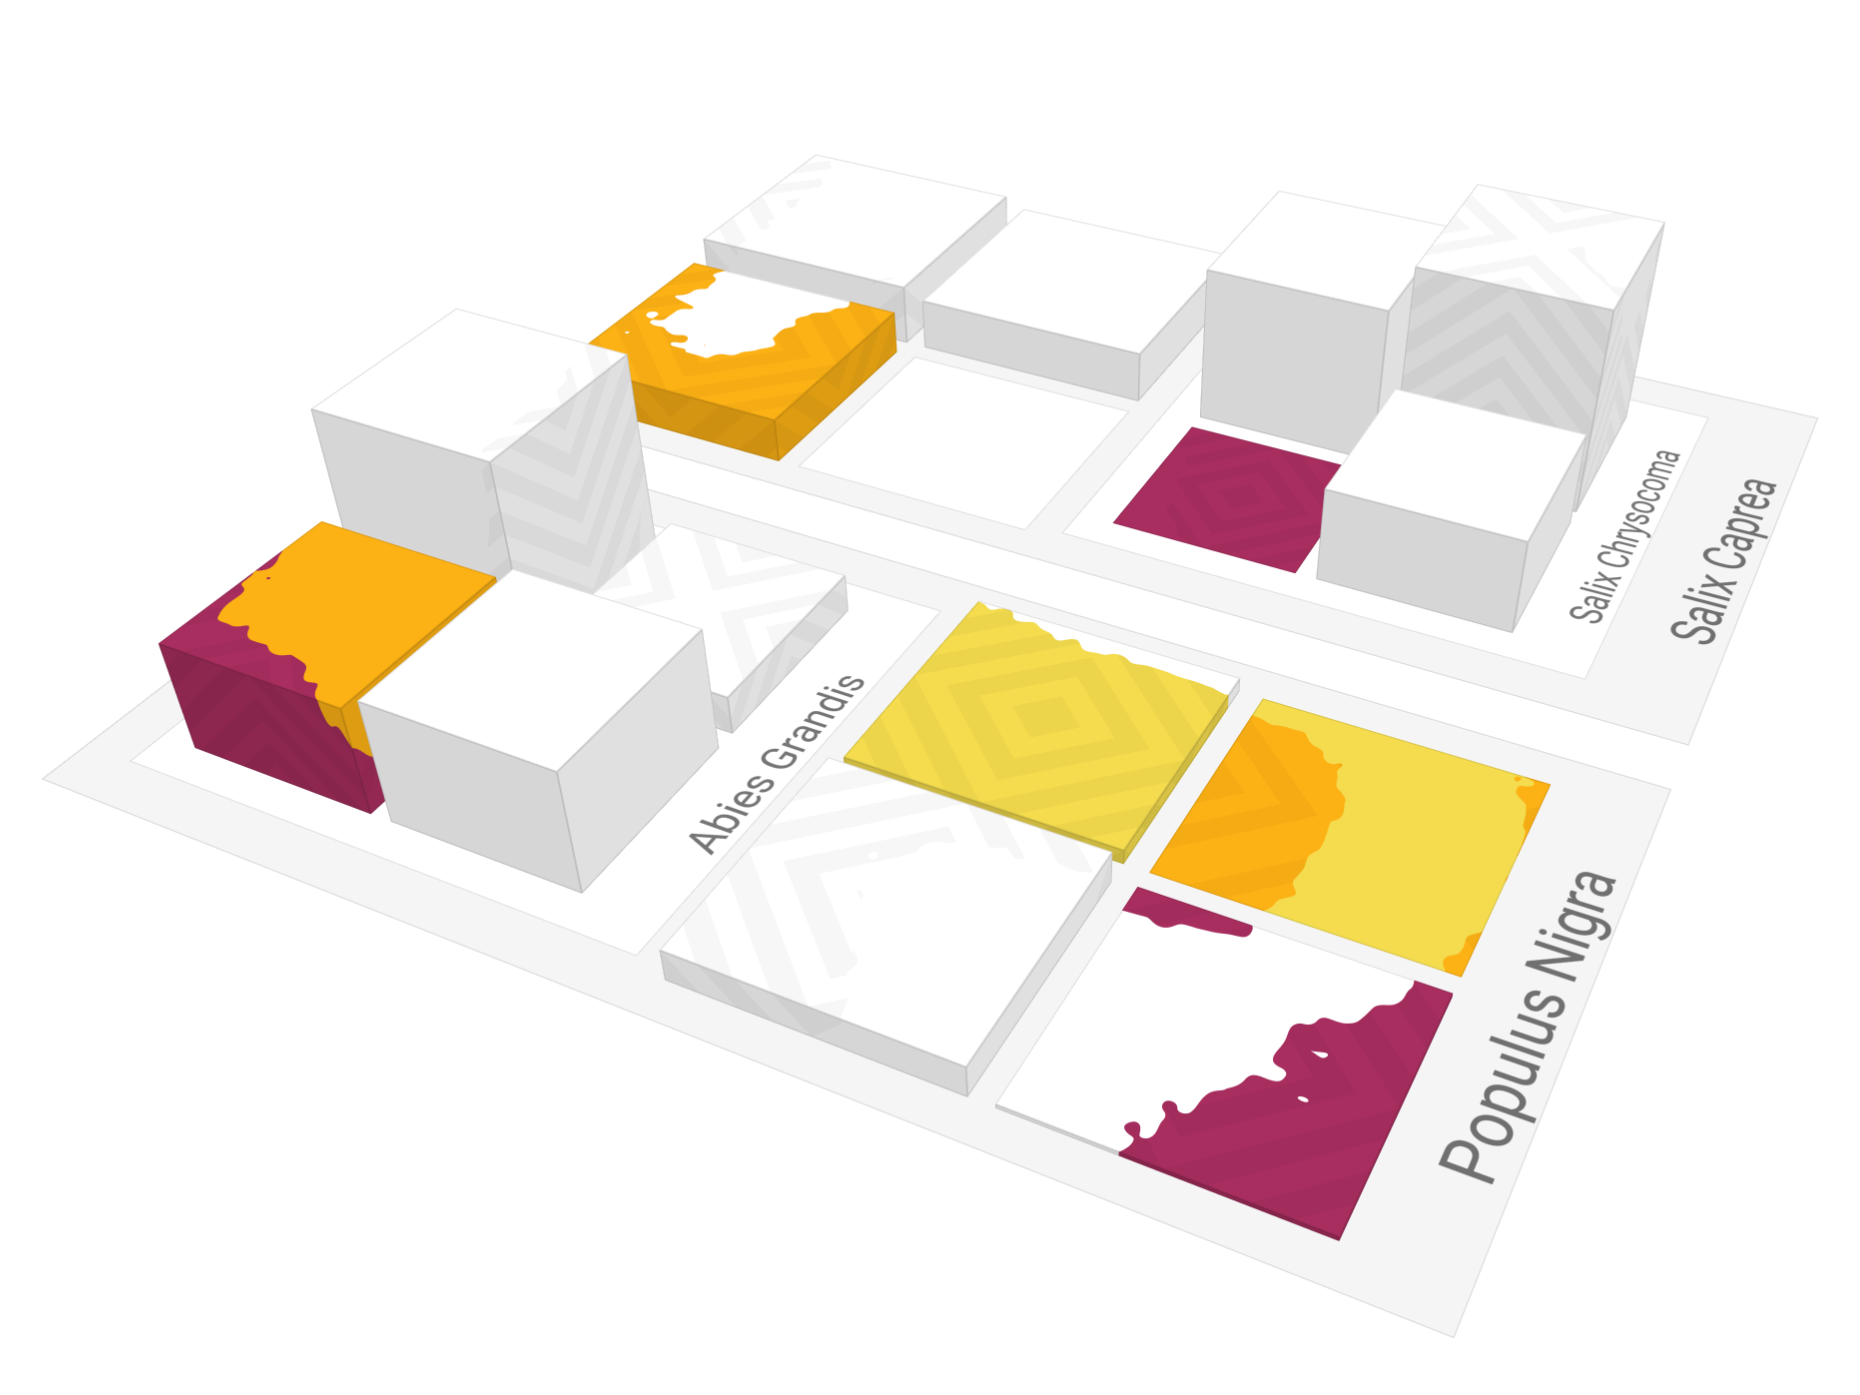
\includegraphics[width = \twffp, trim = 0 0 0 0, clip]{figures/_jov-tasam-teaser-a}};
        \node[figRC, anchor = west](fig1) at ([xshift = \pfull] fig0.east) 
            {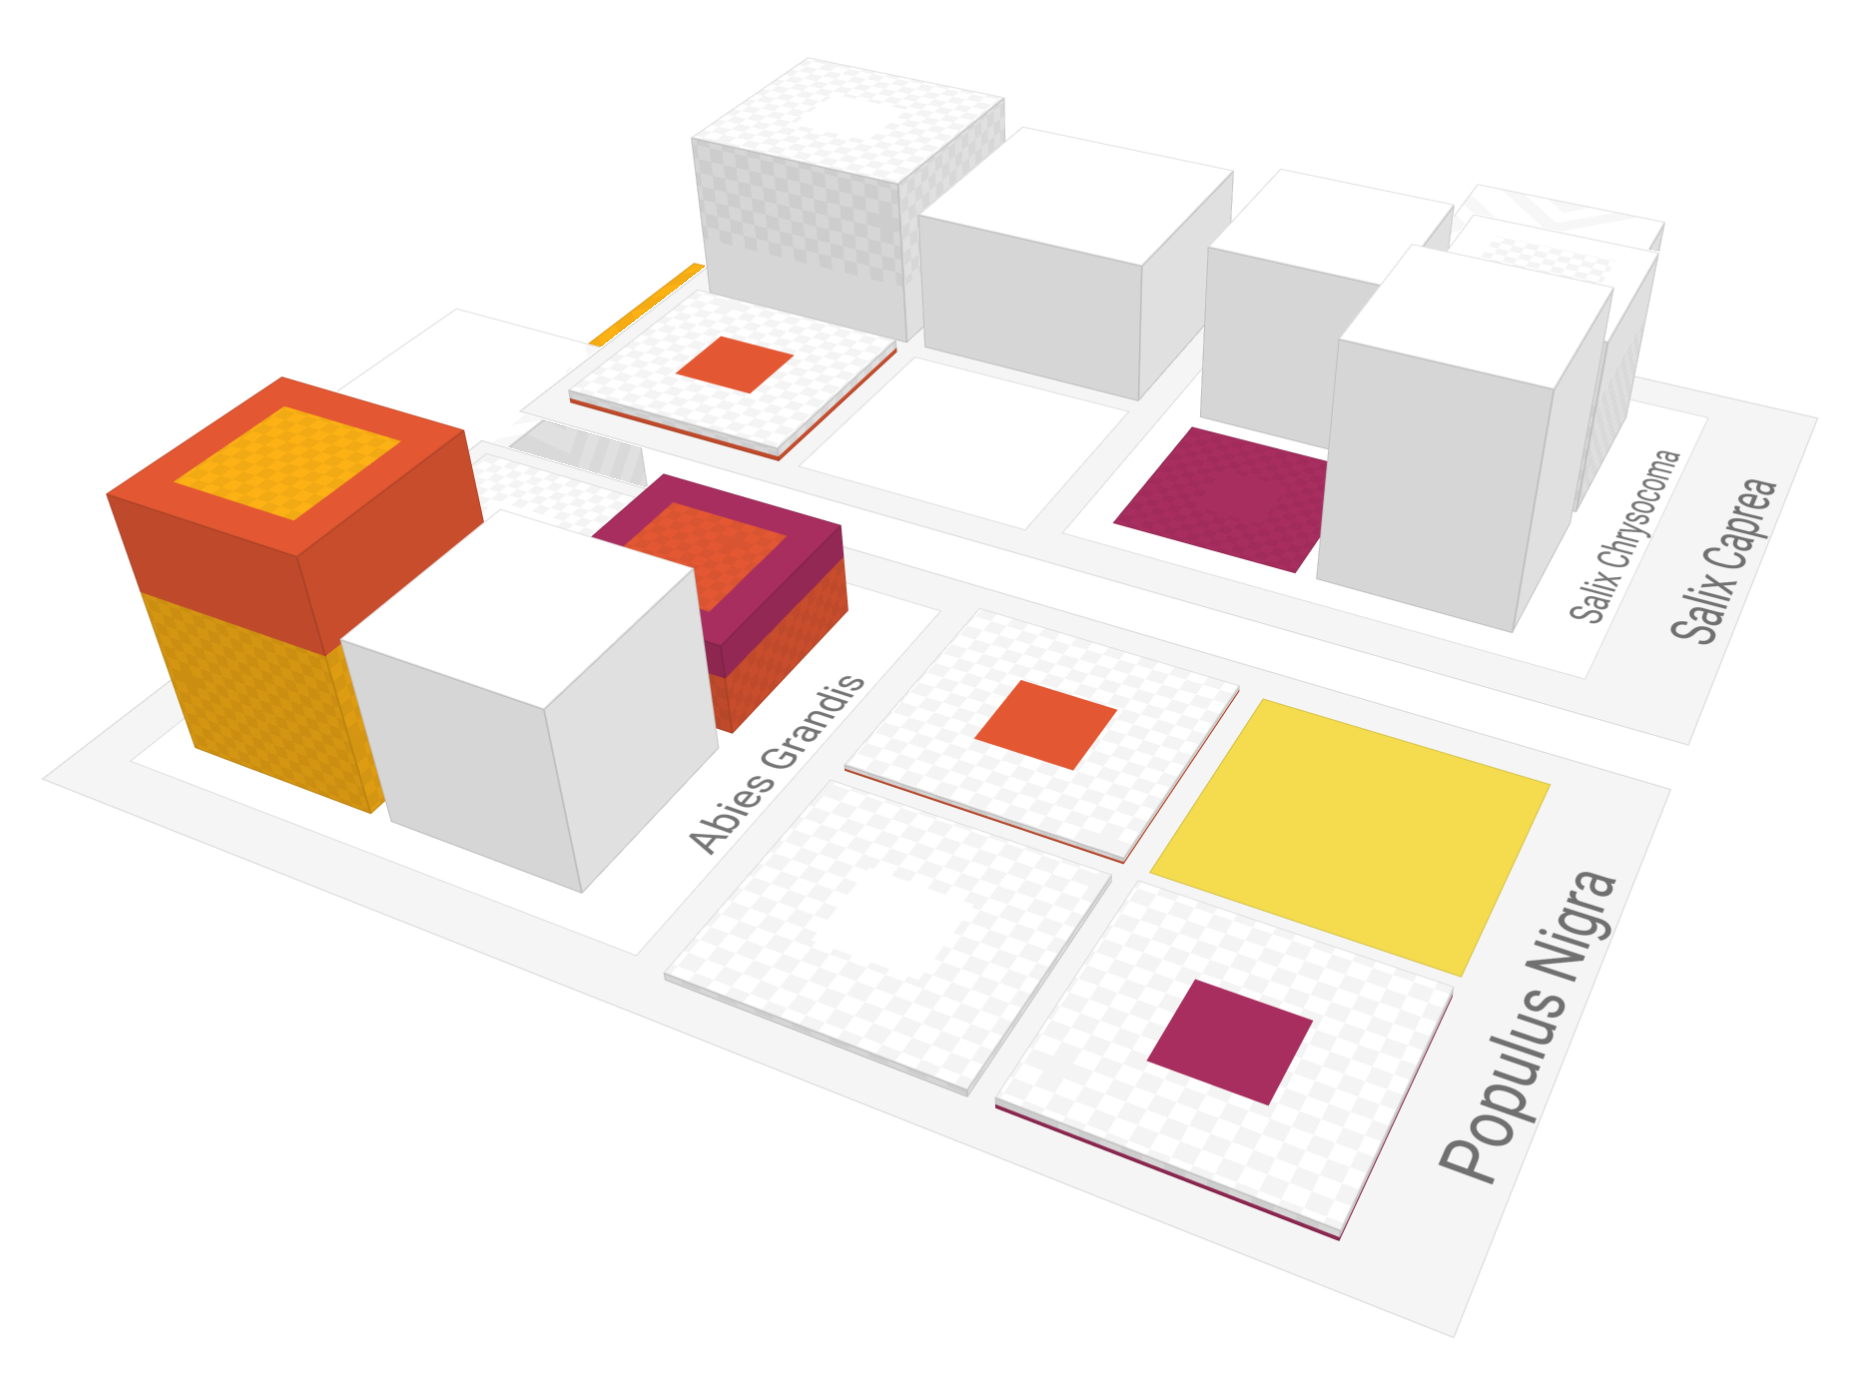
\includegraphics[width = \twffp, trim = 0 0 0 0, clip]{figures/_jov-tasam-teaser-b}};
        \node[below left = 0 of fig0, labelSW](lab0){(a) In between revisions $r_{i-2}$ and $r_{i-1}$};
        \node[below left = 0 of fig1, labelSW](lab1){(b) In between revisions $r_{i-1}$ and $r_{i}$};
        \spy on ($(fig0.center)+(-6.3mm, +10mm)$) in node at ($(fig0.north)+(+14mm,+6mm)$);
        \spy on ($(fig1.center)+(-6.3mm, +10mm)$) in node at ($(fig1.north)+(+14mm,+6mm)$);
    \end{tikzpicture}
    \caption{%
        Synthetic hierarchical test dataset with n revisions is depicted using a 2.5D treemap that supports transitioning between subsequent data revisions mapped to color and height. The two examples (a) and (b) show a combination of two procedural patterns used to animate transitions between revisions.}
    \label{fig:teaser}
\end{figure}

Treemaps allow for the visualization of tree-structured data while supporting mappings to multiple visual variables, including size and color~\citep{johnson1991-spacefilling,carpendale2003-considering}.
They are applied for visualization in domains such as business intelligence and software development and facilitate data observation over time~\citep{roberts2018-businessdata,caserta2011-staticaspects}.
Treemaps can be used in static and interactive contexts, i.e., using static images or interactive clients to support interactive visual analytics tasks.
In contrast to 2D treemaps, their embedding in the third dimension, so-called \emph{2.5D treemaps} or \emph{3D-embedded treemaps}, enable additional data mapping and facilitate a city-like metaphor often suggested for the depiction of software projects~\citep{wettel2008-evolution,schulz2011-implicit,limberger2019-softwaremaps}.
Although different layouting shapes exist for treemaps~\citep{scheibel2020-treemaplayouts}, we focus on the widely used rectangular layouts, and, thus, rectangular 2.5D treemaps.

In order to depict changes in time-varying data,
we use an abstraction of a former and a latter state, whose values should be encoded at their respective nodes.
This can be achieved by depicting the former and latter state using multiple visual variables simultaneously or extending the capabilities of existing ones, e.g., using in-situ representations~\citep{tu2007-changes} or procedural textures.
This idea was recently applied to 2.5D treemaps to depict changes in multiple attributes simultaneously~\citep{limberger2019-insitu}.

When taking advantage of the additional visual variables offered in three dimensions, an important task is to use an effective encoding that allows identifying the former state and the latter state, as well as the magnitude and the direction of a change in values.
We identify these as the \emph{direction of animation}, the \emph{magnitude of change}, and the \emph{direction of change}, respectively.
In the case of the 2D contrast treemap of \citeauthor{tu2007-changes}, this is done by explicit ordering and fixed orientation of the treemap, allowing for an easy-to-replicate reading direction.
For 2.5D treemaps, procedural textures can be used to encode the direction of change for the spatial dimensions, such as a change in height.
However, encoding the direction of change for the color mappings is incompatible with this approach.

In this work, we extend on an earlier work using procedural patterns to depict data changes over time in 2.5D treemaps~\citep{limberger2021-procedural-textures}.
Based on this, we present an approach to design and integrate procedural texture patterns for rectangular 2.5D treemaps with area mapping, height mapping, and color mapping while focusing on communicating changes in color.
The patterns are suitable for both static and interactive application contexts, i.e., used as a static image or during animated transitions, respectively~(\autoref{fig:teaser}).
We showcase the approaches using a prototypical implementation in WebGL that can visualize treemaps with up to hundreds of thousands of nodes.
Extending on the previous work, this includes details on our implementation, further applications, and a discussion.
In summary, our main contributions are:
\begin{itemize}
    \item the concept of procedural texture patterns that are suitable for mapping change in color in rectangular 2.5D treemaps,
    \item a catalog of seven specific patterns as examples to showcase the design space and the trade-off between characteristics,
    \item an extension to include a secondary patterns for accurate display of change direction even for static display of an image,
    \item a detailed description of a prototypical GPU-based implementation with focus on memory layout of per-vertex data and the integration of the procedural textures in fragment shader calls, and
    \item an evaluation of the prototype with focus on performance impact compared to a rendering system without texture pattern capabilities, and two case studies on real-world software projects.
\end{itemize}

The remainder of this paper is structured as follows:
Section~2 presents and discusses related work.
Section~3 introduces procedural textures to extend the color mapping of 2.5D treemaps and a catalog of example patterns.
Section~4 contains evaluation by means of a descriptions of our prototype, the case studies, and a discussion.
Last, section~5 concludes this paper.

\begin{figure}[tb] %
    \begin{tikzpicture}[figNS, spy using outlines = {style = spyRC, darkgray, magnification = 2.25, width = 24mm, height = 14mm}]
        \node[figRC, anchor = south](fig0) at (0,0)
            {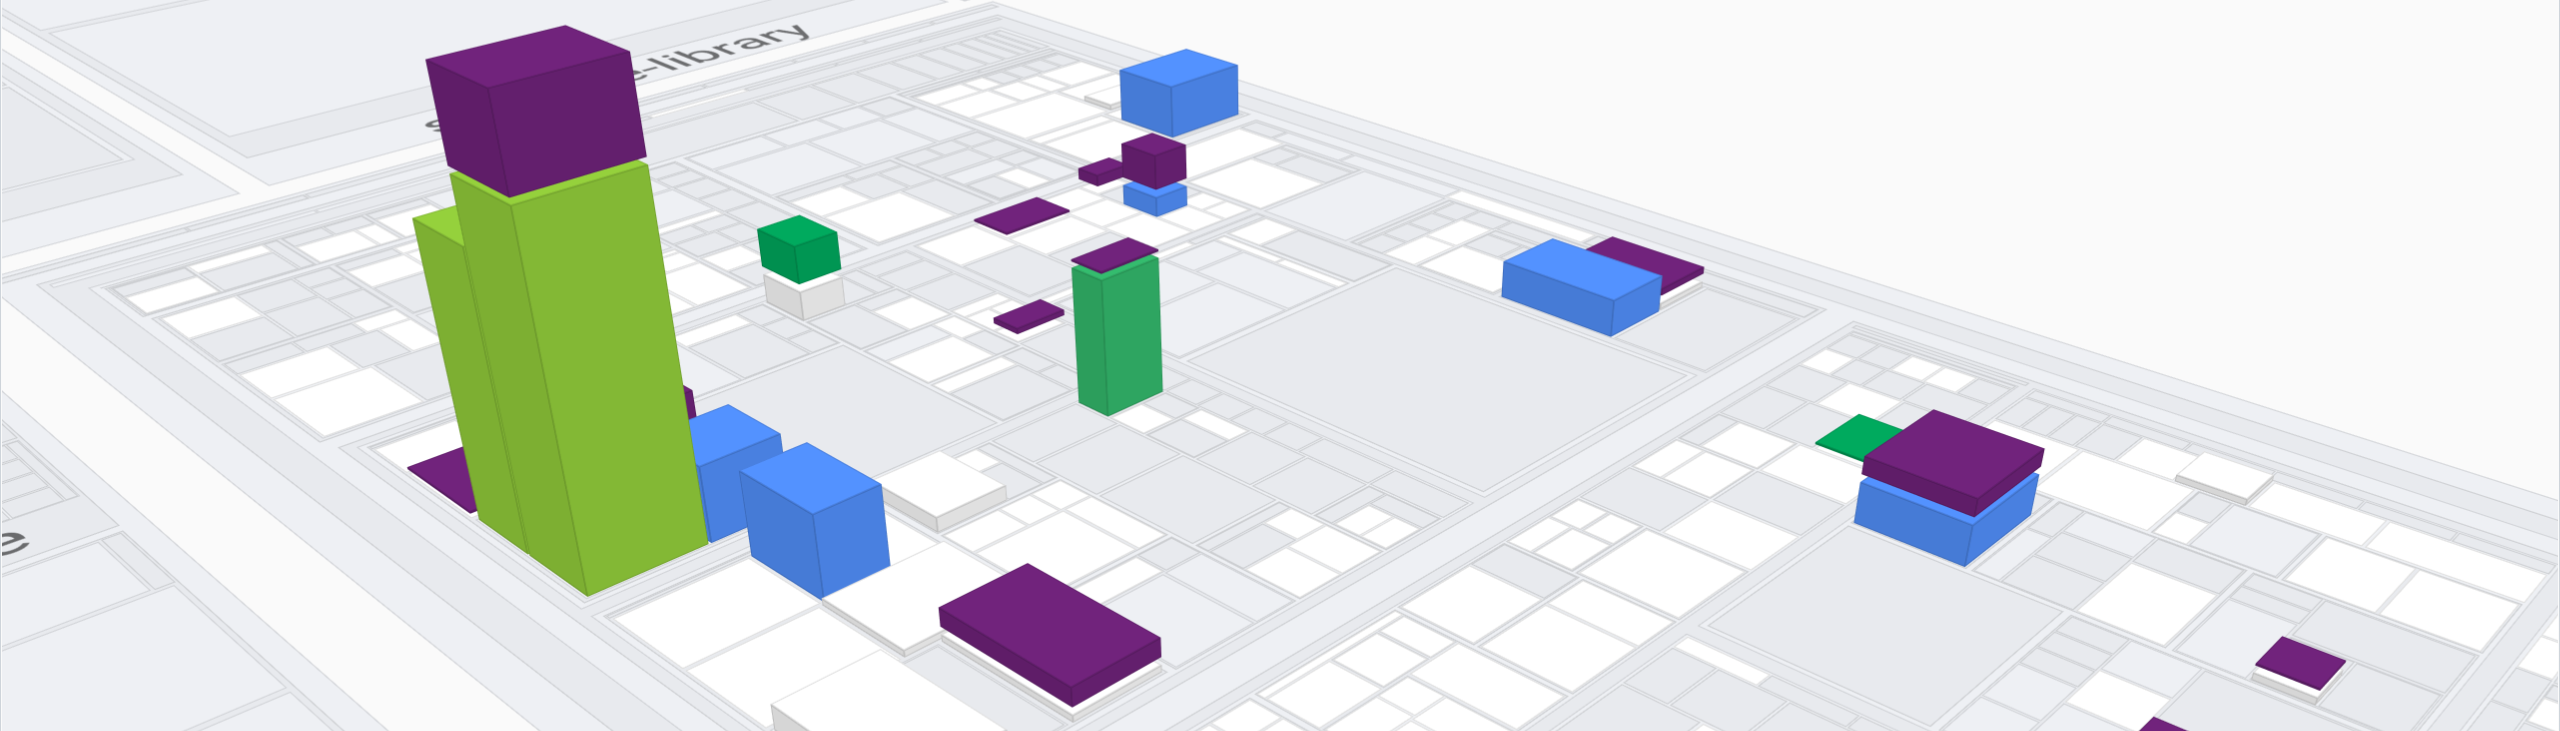
\includegraphics[width = \textwidth, trim = 2 2 2 2, clip]{figures/_jov-diff-classical-stack}};
        \node[figRC, anchor = north](fig1) at ([yshift = -\pfull] fig0.south) 
            {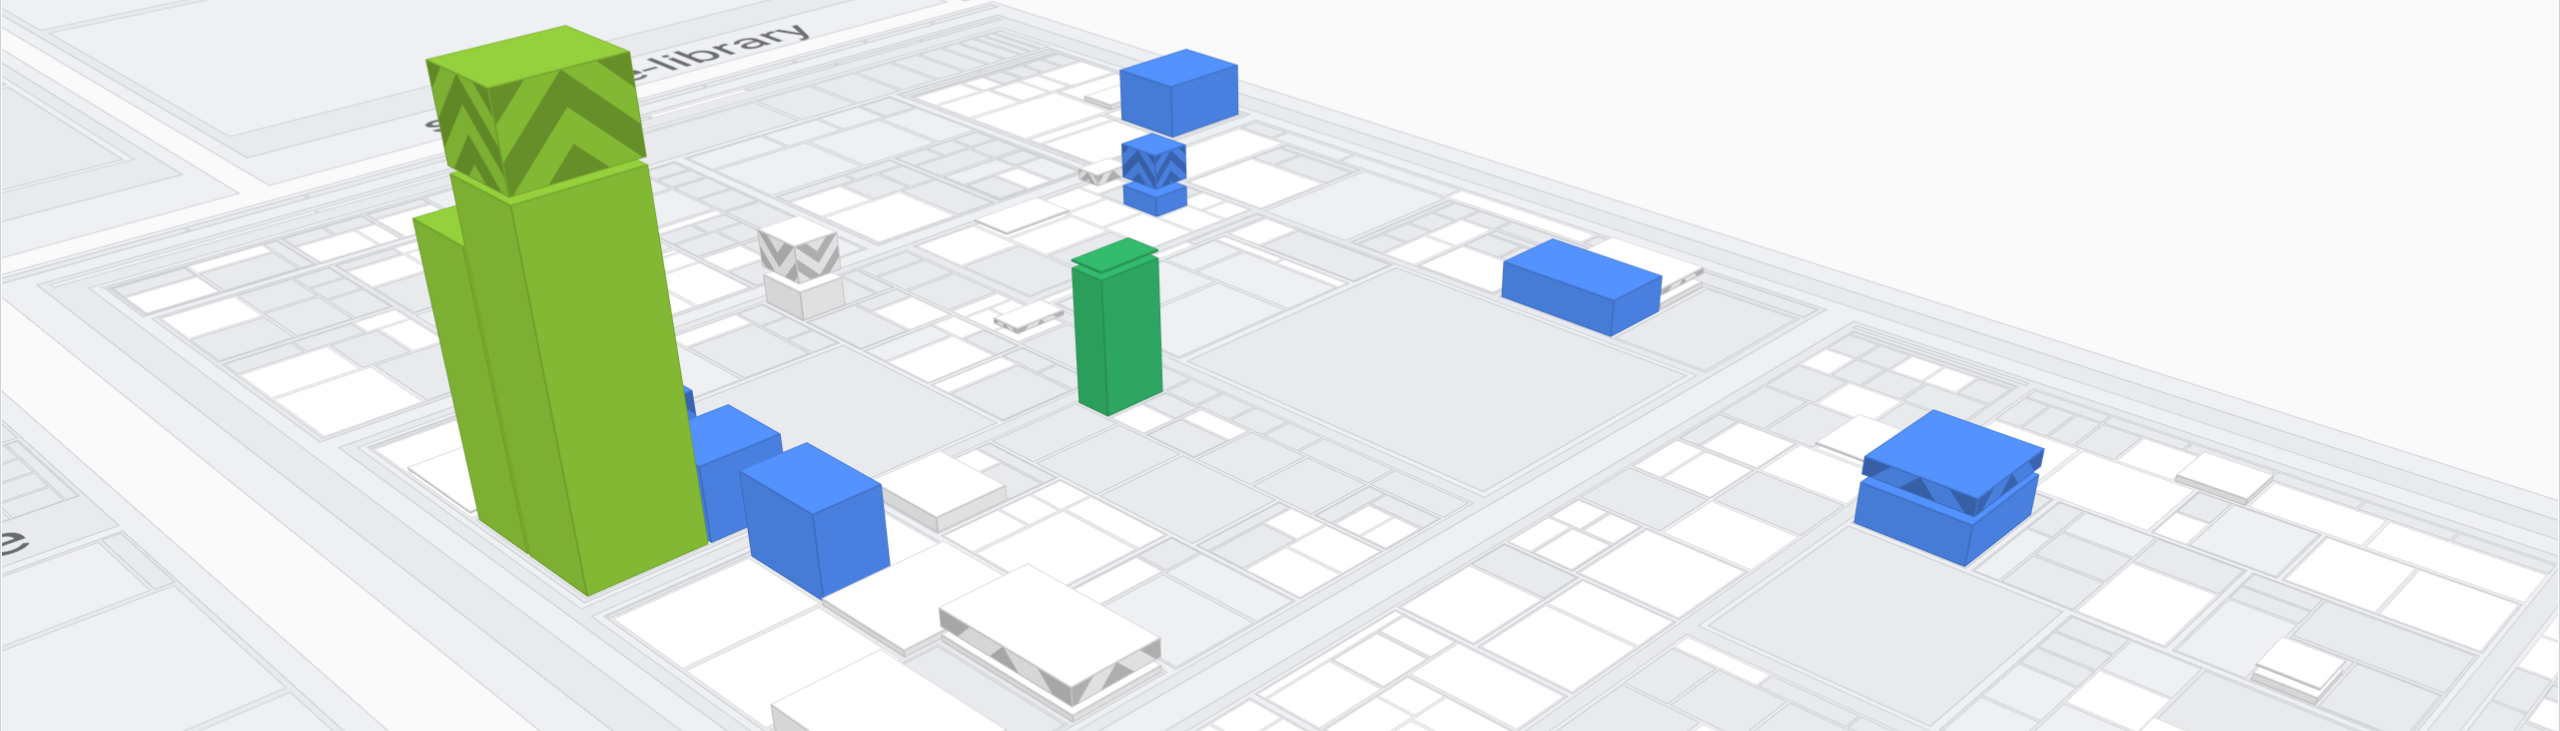
\includegraphics[width = \textwidth, trim = 2 2 2 2, clip]{figures/_jov-diff-classical-arrows}};
        \node[below left = 0 of fig0, labelSW](lab0){(a) Changes in height are color coded (and can be read from the top).};
        \node[below left = 0 of fig1, labelSW](lab1){(b) Changes in height are indicated as down-ward or up-ward oriented arrows.};
        \spy on ($(fig0.center)+(-6mm, +9mm)$) in node at ($(fig0.center)+(+45.5mm,+8mm)$);
        \spy on ($(fig0.center)+(-22mm, +5mm)$) in node at ($(fig0.center)+(+45.5mm,-8mm)$);
        \spy on ($(fig1.center)+(-6mm, +9mm)$) in node at ($(fig1.center)+(+45.5mm,+8mm)$);
        \spy on ($(fig1.center)+(-22mm, +5mm)$) in node at ($(fig1.center)+(+45.5mm,-8mm)$);
    \end{tikzpicture}
    \caption{%
        Basic approaches for communicating changes of subsequent data values mapped to height using colors (top) and arrows (bottom) mapped to the actual difference in height. The former uses a separate color mapping, thereby partially occluding the actual color mapping, and the latter uses procedural patterns for explicit encoding of the change in height and the change direction using an arrow pattern.}
    \label{fig:static-display}
\end{figure}

\section{Related Work}
Depicting change in data is an often-performed mapping in InfoVis and not novel to treemaps.
Although there are more aspects to adopting treemaps for use over time, such as layout stability~\citep{vernier2020-comparison}, we focus on depicting change within this work.
Typically, changes can be depicted using comparative layouts, such as juxtaposition, superposition, explicit encoding, and animated transition~\citep{lyi2020-comparative}.
With software maps, an example application of 2.5D treemaps, we can represent aspects of a software system for a specific revision or time.
We want to enable users to interactively explore correlations in time-varying software system engineering data, e.g., metrics per revision, development budgets, status and progress of defects and issues, team composition, development activity, and others.
This data should be depicted not only for a specific point in time but over time as well.

For example, the time dimension can be incorporated by distributing multiple maps spatially using small multiples~\citep{scheibel2016-smallmultiples,chen2017-pesticide}.
Provided the evolution over more than just two states is already analyzed and available by means of trend data, natural metaphors such as physical-based material degradation or shininess can be an effective tool for communication~\citep{wurfel2016-naturalphenomena}.
Another goal is to augment height and color mappings already in use and rely on the user's existing understanding of treemaps while emphasizing changes in the data.
Thereby, the representation of change should visually correspond to the change in data (\emph{visual-data-correspondence})~\citep{kindlmann2014-algebraic}.
This holds for both the actual difference between two values and the direction of change (or sign of the difference).
For this, basic variants of \emph{data vases}~\citep{thakur2009-datavases} or \emph{in-situ templates}~\citep{limberger2019-insitu} can be used.
The latter allows for change encoding of up to three visual variables, i.e., area, color, and height, simultaneously.
However, reading direction issues must be considered, and ample training is required, too.
An example for the use of in-situ templates to display changes in height is given in~\autoref{fig:static-display}.

These approaches, however, handle the depiction of change in color by increasing the geometric complexity.
In contrast, we extend on approaches that encode the change into the existing geometric representation.
For 2D treemaps, color patterns such as \emph{two corners}, resulting in a diagonal color gradient, or contrast modifications like \emph{ratio shading} can be used for 2D treemaps~\citep{tu2007-changes}.
Regarding 2.5D treemaps, animation using an interpolation of height and color attributes could be used, too~\citep{bladh2005-transitions,langelier2008-evolution}.
With our focus on changes in data mapped to color, our approach is also related to encoding multiple colors within the same surface or space, known as color weaving~\citep{urness2003-multi-valued}, which was also applied to visualize two measures in color on treemaps~\citep{benomar2013-dynamicities}.
For this weaving, the effectiveness of reconstructing the ratio of colors as a user was examined for 2D visualizations~\citep{haghshenas2007-weaving}.

\section{Procedural Texture Patterns}
For a rectangular 2.5D treemap, a cuboid's top face and lateral faces are typically used for single-value color mapping, which we use to superimpose a second color representing a second value.
For that, we use the concept of transition-aware texture patterns that are procedurally generated using \emph{procedural textures} in computer graphics~\citep{Quilez13}.
These texture patterns are applied to the top and lateral faces and allow to show both colors on a cuboid's surface.
Such a pattern maps a distribution of two colors onto a surface without introducing additional colors.

Let $C = [0,1]^3 \subseteq \mathbb{R}^3$ denote the unit cube in the Euclidean space $\mathbb{R}^3$ that is used to provide a local parameterization of a treemap node.
Its surface $S$ is given by the boundary of $C$, i.e., $S = \partial C$. 
A pattern on the surface $S$ is a function given by 
\begin{align*}
    P: S \times [0,1] \to \{c_f, c_l \}, (p, \lambda) \mapsto P(p, \lambda) = P_{\lambda}(p),
\end{align*}
where $\lambda \in [0,1]$ is called progress value and $c_f$ and $c_l$ are two colors representing the value of the former state and the latter state.
Furthermore, a pattern $P$ satisfies the following three properties:
\begin{enumerate}
    \item $\area(\{P_0 = c_l \}) = 0$,
    \item $\area(\{P_1 = c_l \}) = \area(S)$, and
    \item  $\forall \lambda_1, \lambda_2 \in [0,1]: \lambda_1 < \lambda_2 \implies \area(\{P_{\lambda_1} = c_{l}\}) \leq \area(\{P_{\lambda_2} = c_{l}\})$,
\end{enumerate}
where $\area$ denotes the usual area of surface in $\mathbb{R}^3$ and the set $\{P_{\lambda} = c_{l}\}$ denotes the subset points on $S$, where the pattern takes the value $c_l$.

As specific examples of such transition-aware texture patterns, we propose seven patterns, namely (1) Pillar, (2) Pyramid, (3) Arrows, (4) Arrows (full), (5) Noise, (6) Dithering, and (7) Squares (\autoref{fig:trans-vars}).
As the proposed patterns share approaches but also differ in their visual display and characteristics, we propose a set of characteristics to capture their abilities for information encoding.
Further, we propose an extension to superimpose two patterns to enhance the direction of change for static images.
In an interactive context, this progress value $\lambda$ should gradually increase from $0$ to $1$, resulting in an animated transition.
In static contexts, this value can be chosen constant, e.g., the progress value $\lambda = \nicefrac{1}{2}$ that represents half the transition.

\subsection{Pattern Characteristics}
A mapping from a progress value to the color distribution of two colors on a surface brings a number of optimization possibilities.
We focus on five desirable characteristics that try to capture what a pattern can visually \emph{encode} and how this pattern transforms during animated transitions, i.e., the more a texture pattern supports, the more it should be suitable for mapping change onto color.
They are designed to capture whether a pattern can discern the former and the latter color (read direction), and the current transition progress value.
Additionally, we add four characteristics that attribute \emph{compatibility}. 
As such, they support applications of the texture patterns to treemaps in other contexts and differing parameterizations, e.g., the combination with other visual variable mappings and their potential animated transition, or choice of the base shapes for layouting.
The encoding characteristics are as follows:
\newlength{\maxlabel}
\setlength{\maxlabel}{\widthof{$\nabla_{\textrm{Polygonal}}$}+0.5em}
\begin{description}[itemindent=0mm,labelwidth=0mm,leftmargin=\maxlabel,align=right,itemsep=1mm]
    \item [$\nabla_{\textrm{Monotonic}}$]
        A pattern is \emph{monotonic} if a point of the surface switches from displaying the former color to the latter color only once. We only propose patterns in the catalog that have this characteristics. Patterns that are not \emph{monotonic} introduce flickering into an animated transition.
    \item [$\nabla_{\textrm{DirStates}}$]
        This characteristic measures whether the two encoded states can be read unambiguously, i.e., discerning the former from the latter state, in a static image or while the animation is paused during a transition.
        Further, this takes different viewpoints of the user as well as potential occlusion of parts of a cuboid into account.
    \item [$\nabla_{\textrm{DirChange}}$]
        The direction of change in value, increase or decrease, can be read unambiguously in a static image or while the animation is paused during a transition.
        This also takes different viewpoints as well as potential occlusion of parts of a cuboid into account.
    \item [$\nabla_{\textrm{RatioLat}}$]
        The ratio of different colors on the lateral faces matches a transition's progress.
        These lateral faces' area scales with the value mapped to height and partially with the value mapped to weight.
    \item [$\nabla_{\textrm{RatioTop}}$]
        The ratio of different colors on the top face matches a transition's progress (top view or 2D treemap).
        The top face area scales with the value mapped to weight.
\end{description}
The compatability characteristics are as follows:
\begin{description}[itemindent=0mm,labelwidth=0mm,leftmargin=\maxlabel,align=right,itemsep=1mm]
    \item [$\nabla_{\textrm{IndHeight}}$]
        The mapping of change difference and change direction does not compromise the height mapping as well as a display of change mapped to height.
    \item [$\nabla_{\textrm{IndWeight}}$]
        The mapping of change difference and change direction does not compromise the weight mapping as well as a display of change mapped to weight.
    \item [$\nabla_{\textrm{TreeSize}}$]
        The pattern can be easily adjusted for large or very large treemaps.
        This characteristic holds, if for a range of treemap sizes, the pattern can be read in a meaningful way, i.e., all other characteristics are retained.
    \item [$\nabla_{\textrm{Polygonal}}$]
        The pattern is suitable to be applied to treemaps with general polygonal shapes.
        This includes that the pattern's visual metaphor upholds and an implementation is identical or similar to the rectangular one.
\end{description}

\begin{figure}[tbp]
    \begin{tikzpicture}[figNS, spy using outlines = {style = spyRC, darkgray, magnification = 2.25, size = 32}]
        \matrix[column sep=1em, row sep=1.5em] {
            \node[] { Pillar }; &
            \node[anchor=west](arrows0) {%
                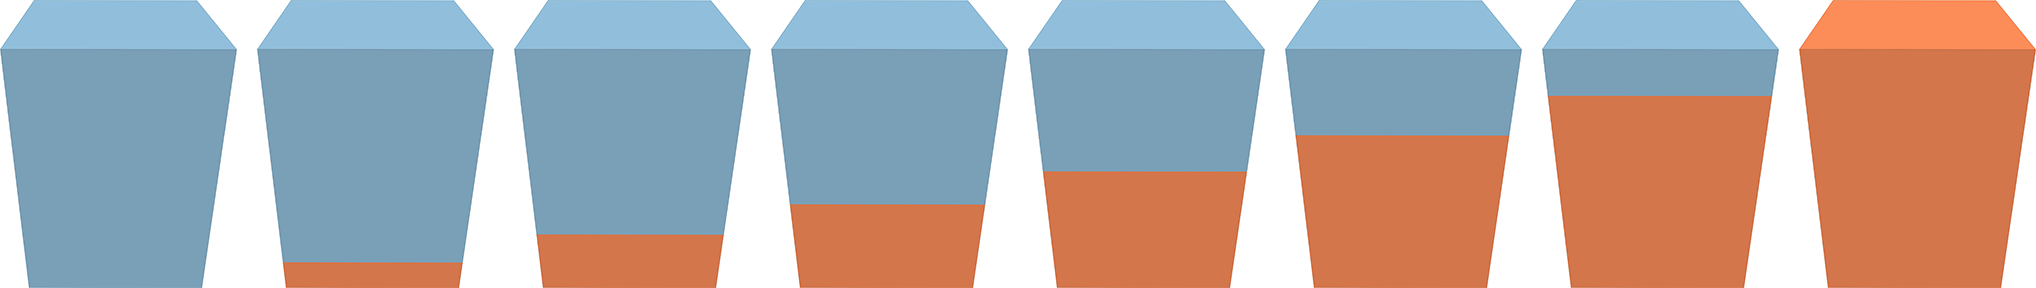
\includegraphics[width=0.85\linewidth]{figures/basic-trans-vars-vertical}}; \\
            \node[] { Pyramid }; &
            \node[anchor=west](arrows1) {
                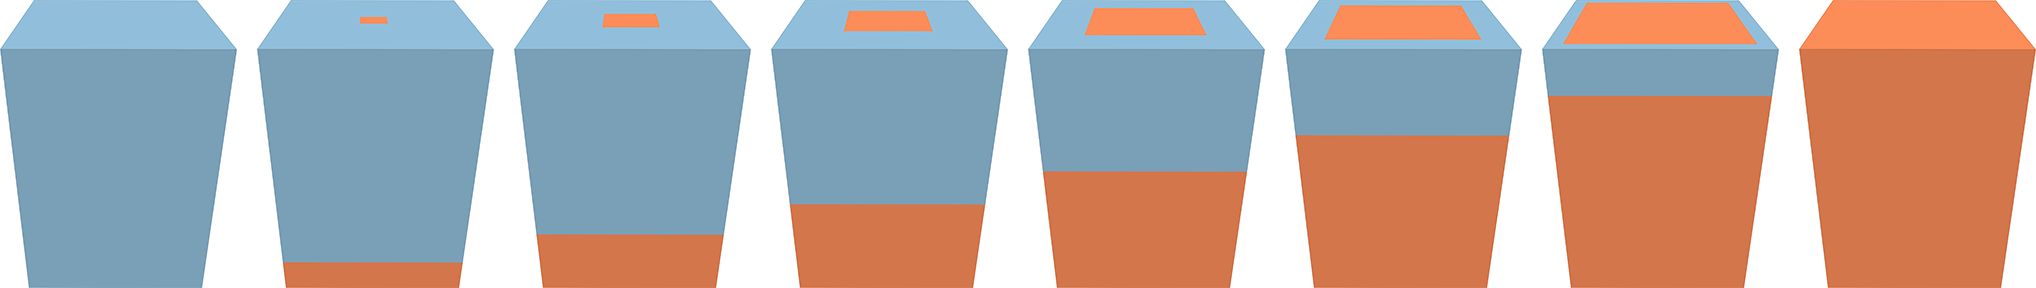
\includegraphics[width=0.85\linewidth]{figures/basic-trans-vars-pyramid}}; \\
            \node[] { Dithering }; &
            \node[anchor=west](arrows2) {
                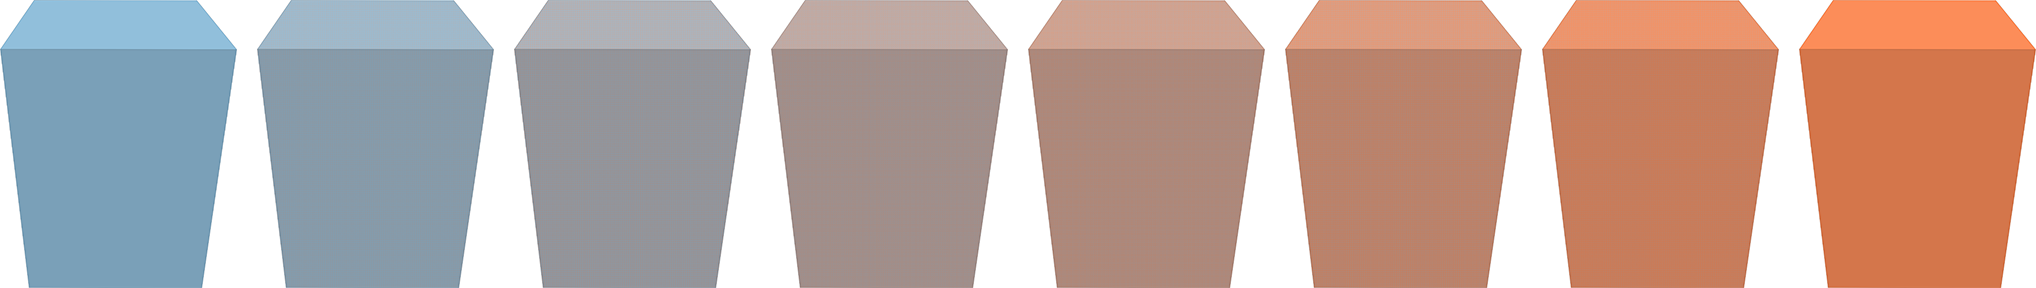
\includegraphics[width=0.85\linewidth]{figures/basic-trans-vars-dithering}}; \\
            \node[] { Squares }; &
            \node[anchor=west](arrows3) {
                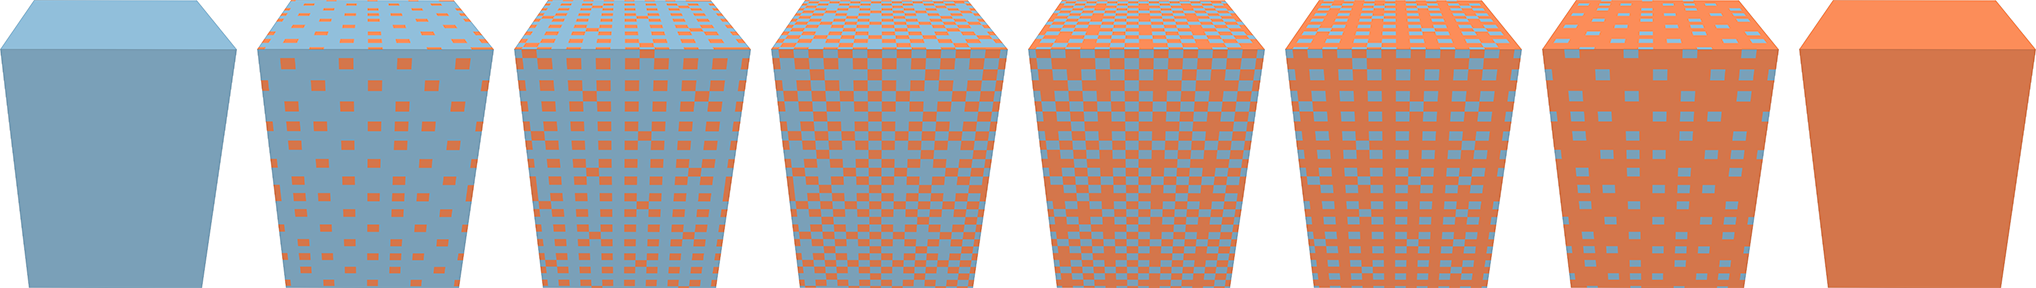
\includegraphics[width=0.85\linewidth]{figures/basic-trans-vars-quads}}; \\
            \node[] { Noise }; &
            \node[anchor=west](arrows4) {
                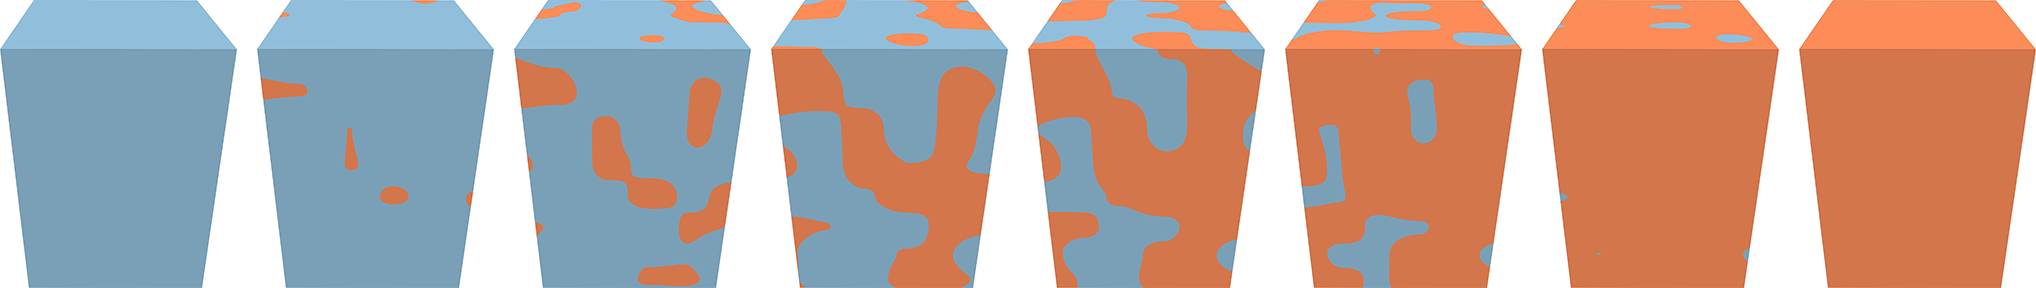
\includegraphics[width=0.85\linewidth]{figures/basic-trans-vars-noise}}; \\
            \node[] { Arrows }; &
            \node[anchor=west](arrows5) {
                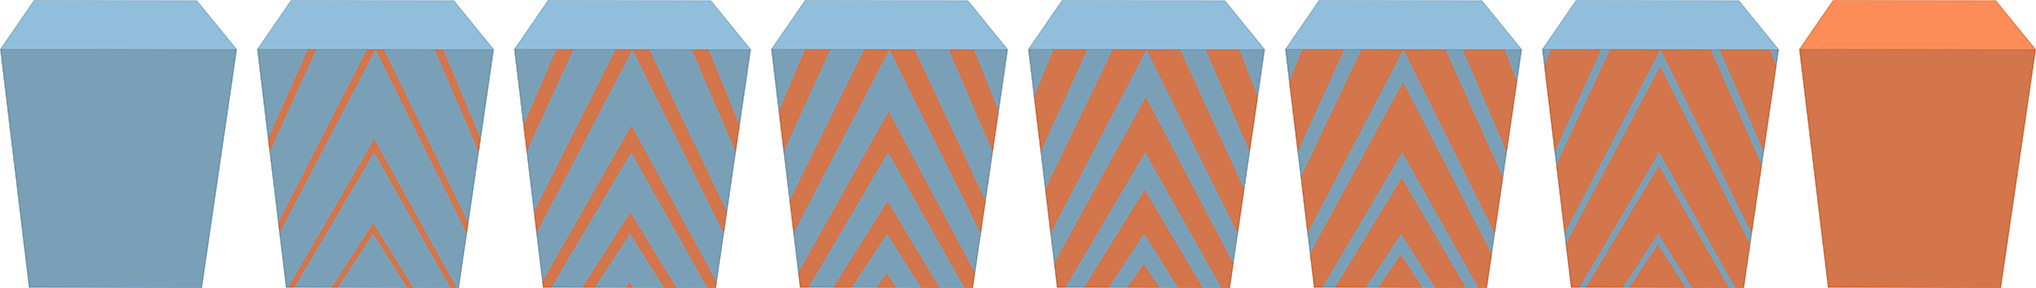
\includegraphics[width=0.85\linewidth]{figures/arrow-trans-vars}}; \\
            \node[] { Arrows (full) }; &
            \node[anchor=west](arrows6) {
                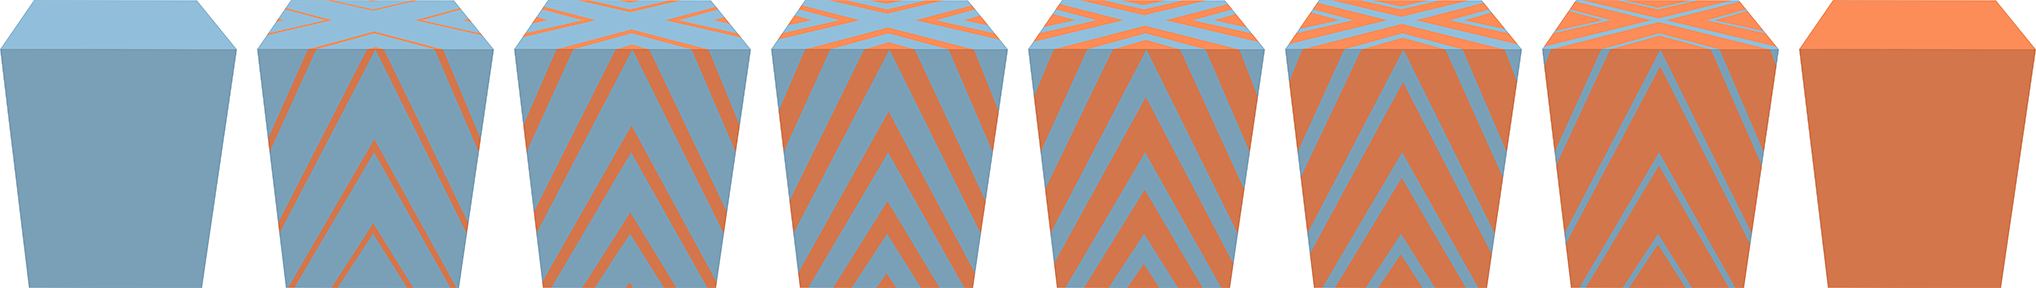
\includegraphics[width=0.85\linewidth]{figures/arrow-trans-vars-variants-full}}; \\
        };
        \spy on ($(arrows2.center)+(+0.45, +0.4)$) in node at ($(+2.0, +0.25)+(arrows2.center)$);
        \spy on ($(arrows3.center)+(+0.45, +0.4)$) in node at ($(+2.0, +0.25)+(arrows3.center)$);
        \spy on ($(arrows4.center)+(+0.45, +0.4)$) in node at ($(+2.0, +0.25)+(arrows4.center)$);
        \spy on ($(arrows5.center)+(+0.45, +0.4)$) in node at ($(+2.0, +0.25)+(arrows5.center)$);
        \spy on ($(arrows6.center)+(+0.45, +0.4)$) in node at ($(+2.0, +0.25)+(arrows6.center)$);
        \node[above left=1em and 1em of arrows0.north west,anchor=south east] {$t = $};
        \node[above=1em of arrows0.north west,anchor=south west] (zero) {0};
        \node[above=1em of arrows0.north east,anchor=south east] (one) {1};
        \draw[very thin,|-latex,shorten <= 1em,shorten >= 1em] (zero) -- (one);
    \end{tikzpicture}
    \caption{
        Procedural patterns for changes in color attribute, from top to bottom: Pillar, Pyramid, Dithering, Squares, Noise, Arrows, and Arrows (full).%
    }
    \label{fig:trans-vars}
\end{figure}

\subsection{Texture Patterns Catalog}
More technically, a texture pattern describes a visual mapping of transition progress for a fragment on a cuboid's surface using a binary per-fragment choice of color for a treemap node's former and latter state.
Each pattern is designed to encode the transition progress by the area ratio of the two colors of the two depicted states.
The seven patterns are a starting point and by no means a complete list of alternatives.
Thereby, each pattern is not precisely defined by a specific implementation or a fragment-precise definition of the binary decision to be made but represents the overall appearance with alternatives and additional parameters.

\paragraph{Pillar.}
The Pillar pattern partitions the surface vertically and assigns the former and latter colors to a top share and a bottom share of the pillar, respectively.
This pattern's transition starts with a full pillar using the former color.
Then, the next color \emph{grows} from the top and overlays the former color step by step.
Thus, after a brief training period, a user should be able to determine the former color and the latter color, even for a static display.
However, this pattern does not show partial progress on the top faces.
Instead, the color of the top face changes instantaneously with the completion of the transition.

\paragraph{Pyramid.}
The Pyramid pattern extends the Pillar pattern by explicitly handling the top faces.
The lateral faces use the same encoding.
However, the name \emph{pyramid} describes the metaphorical process that is used to derive an implementation of the pattern: 
a virtual pyramid is embedded in the cuboid and slowly pushed towards and through the top. 
All cuboid fragments that intersect with the pyramid are assigned the latter, upcoming color.
This intersection surface corresponds to the progress of the Pillar pattern for lateral faces and results in a growing rectangle for top faces.
As a result, this pattern encodes transition progress on both the lateral faces and the top face.

\paragraph{Noise.}
The Noise pattern uses 3D noise~\citep{Perlin01} and a threshold to partition the surface for the two colors.
This results in organic-looking surfaces and transition behavior.
However, a suitable parameterization of the noise with respect to the scaling is challenging.
We propose approximating the scale factor by the number of nodes in the tree  as this measure loosely corresponds to the share of footprint area one node has in relation to the size of the whole treemap.

\paragraph{Dithering.}
The Dithering pattern encodes the transition using a per-fragment dithering pattern.
Dithering is applied in screen space regardless of the orientation of the cuboid.
From a perceptional point of view, this results in a visual blending of the two colors~\citep{Ulichney88}---most likely, the medium on which this paper is read will not be able to display the separated colors.
However, we assert that only actual colors from a color scheme will be used using dithering.

\paragraph{Squares.}
The Squares pattern extends the dithering by using a Dithering pattern that can be scaled for the cuboid's size.
The pattern is applied to the surface in world space, not the display pixels.
Furthermore, it is directly affected by the cuboid's orientation.
This reduces the visual blurring of colors while providing a transition nonetheless.
From an implementation's point of view, designing the overhang from a square onto neighboring surfaces is challenging.
A straightforward approach is to arrange the squares and loosen their aspect ratio to create rectangles such that no overhang occurs.

\paragraph{Arrows.} %
This pattern generates the resemblance of arrows of alternating colors.
The top faces behave similarly to the Pillar pattern.
In contrast to the Pillar and Pyramid patterns, the arrow direction can encode the direction of change in value, as the arrows can point upwards.
Likewise, the pattern can be inverted to resemble downward facing arrows.
These visual cues for the direction of change, however, prevents effective encoding of the direction of the animation.
An extension to this pattern that includes the top face is presented with the Arrows (full) pattern.

\begin{figure}[tb]
    \begin{tikzpicture}[figNS, spy using outlines = {style = spyRC, darkgray, magnification = 2.25, size = 32}]
        \matrix[column sep=1em, row sep=1.5em] {
            \node[anchor=west](arrows0) {
                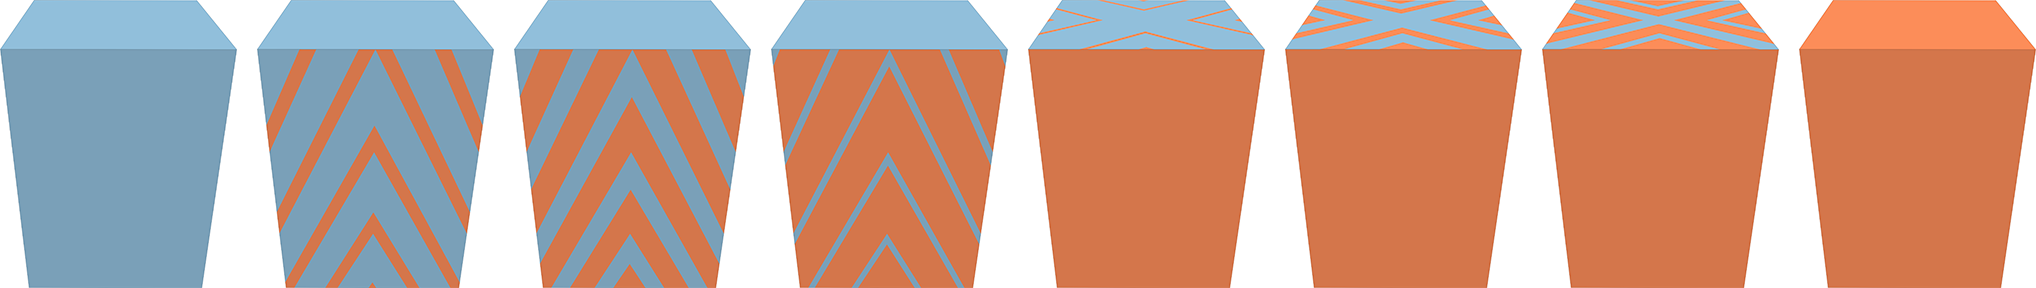
\includegraphics[width=0.85\linewidth]{figures/arrow-trans-vars-variants-divided}}; \\
            \node[anchor=west](arrows1) {
               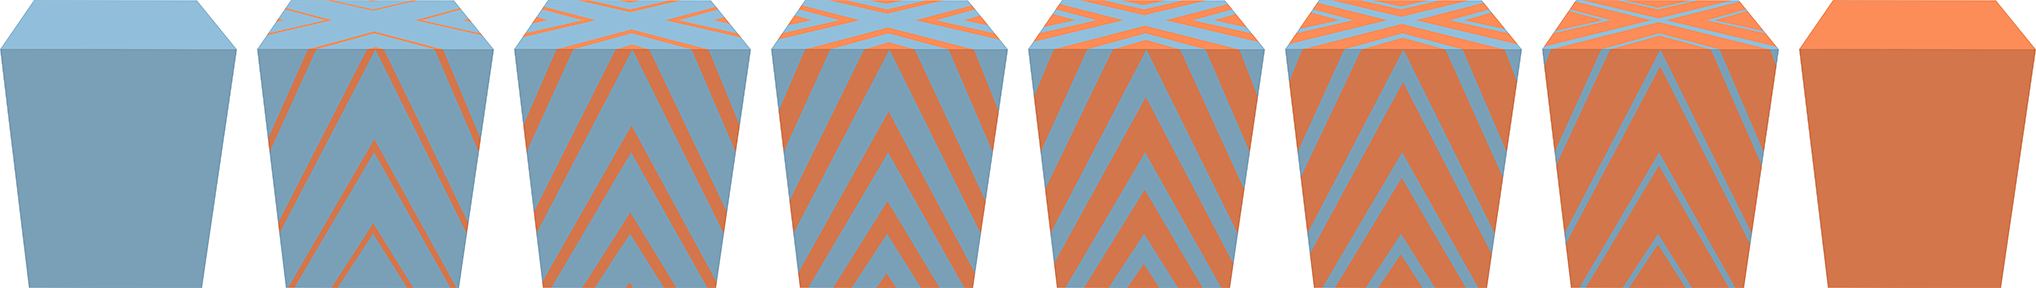
\includegraphics[width=0.85\linewidth]{figures/arrow-trans-vars-variants-full}}; \\
            \node[anchor=west](arrows2) {
               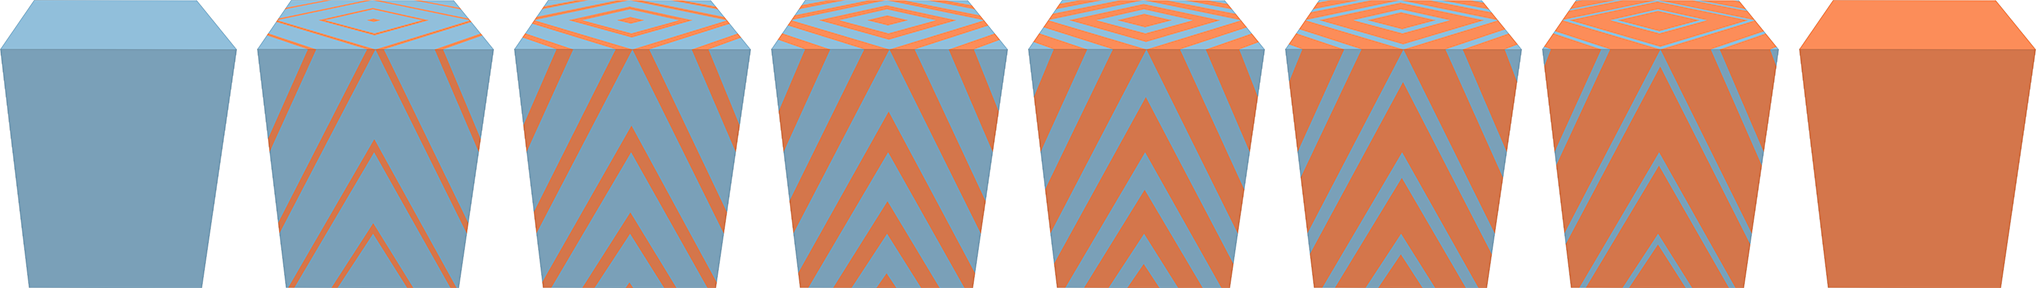
\includegraphics[width=0.85\linewidth]{figures/arrow-trans-vars-variants-full-inverse}}; \\
        };
        \spy on ($(arrows0.center)+(+0.45, +0.4)$) in node at ($(+2.0, +0.25)+(arrows0.center)$);
        \spy on ($(arrows1.center)+(+0.45, +0.4)$) in node at ($(+2.0, +0.25)+(arrows1.center)$);
        \spy on ($(arrows2.center)+(+0.45, +0.4)$) in node at ($(+2.0, +0.25)+(arrows2.center)$);
        \node[above left=1em and 1em of arrows0.north west,anchor=south east] {$t = $};
        \node[above=1em of arrows0.north west,anchor=south west] (zero) {0};
        \node[above=1em of arrows0.north east,anchor=south east] (one) {1};
        \draw[very thin,|-latex,shorten <= 1em,shorten >= 1em] (zero) -- (one);
    \end{tikzpicture}
    \caption{
        Variants of the arrow-pattern transition for increasing values: lateral face first, then top face (top), or lateral and top faces simultaneously (center and bottom).
        Note that the bottom transition uses an inverted pattern for the top to indicate a value increase when seen from above.
    }
    \label{fig:arrow-trans-vars-variants}
\end{figure}

\paragraph{Arrows (full).}
This pattern extends the Arrow pattern by additional arrows on the top face.
As with the Arrow pattern, the arrows can be inverted, too, to encode the direction of change.
However, the direction of the arrows on the lateral surfaces and the additional top surface allows for additional design considerations (\autoref{fig:arrow-trans-vars-variants}).
For one, they can be appended to the transition of the lateral faces, i.e., the transition starts with arrows on the lateral faces and ends with arrows on the top face.
This allows encoding of direction on top only for a short duration of the transition.
Alternatively, the arrows can be animated simultaneously on the top faces for the whole duration of the transition, whereby two variants with opposite directions are available.
However, both directions, (1) the visual extension to the arrow-forming stripes from the lateral surfaces, and (2) individual arrows, pose non-intuitive reading along the lateral and top face border.

\subsection{Pattern Composition}
Although some patterns can encode the semantics of direction of change, invariant to all patterns is that the direction of animation and the direction of change value can be encoded simultaneously.
As an additional indicator for the direction of animation, we propose to superimpose two different patterns.
One of the two distinctly colored areas is filled with a pattern instead of a solid color~(\autoref{fig:trans-vars-combinations}).
This allows for a direct, unambiguous display of change direction when paused and animated, as only one state has a second pattern superimposed.
This pattern remains constant during the transition, e.g., reusing any other pattern with $\lambda = \nicefrac{1}{2}$.
However, as the overall transition changes the surfaces encoding former and latter colors, the area of the secondary pattern will vary during the transition.

\begin{figure}[tb]
    \begin{tikzpicture}[figNS, spy using outlines = {style = spyRC, darkgray, magnification = 2.25, size = 32}] \matrix[column sep=1em, row sep=1.5em] {
            \node[anchor=west](arrows0) {
                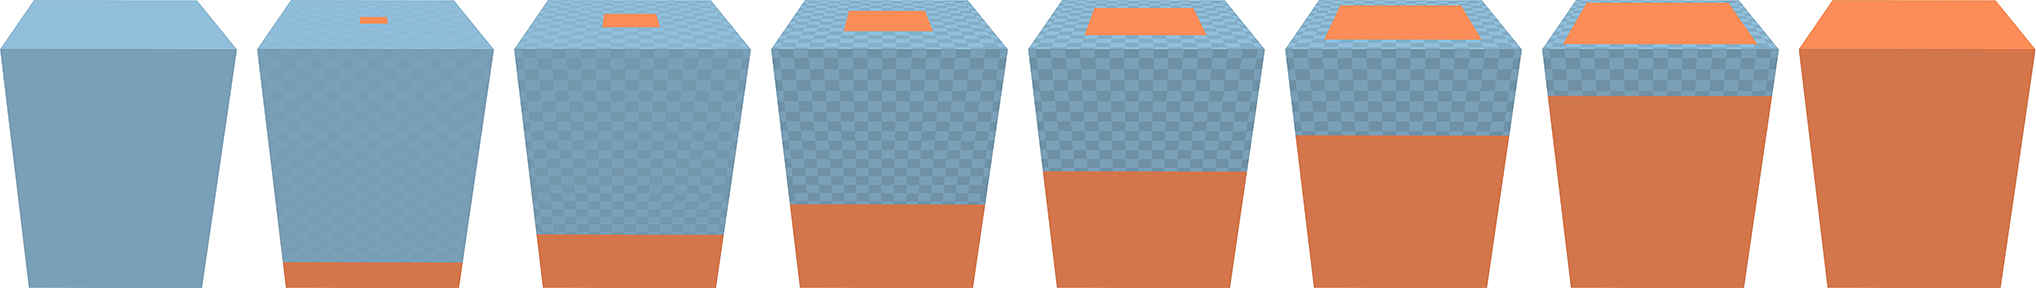
\includegraphics[width=0.85\linewidth]{figures/trans-vars-combinations-pyramid-quads}}; \\
            \node[anchor=west](arrows1) {
               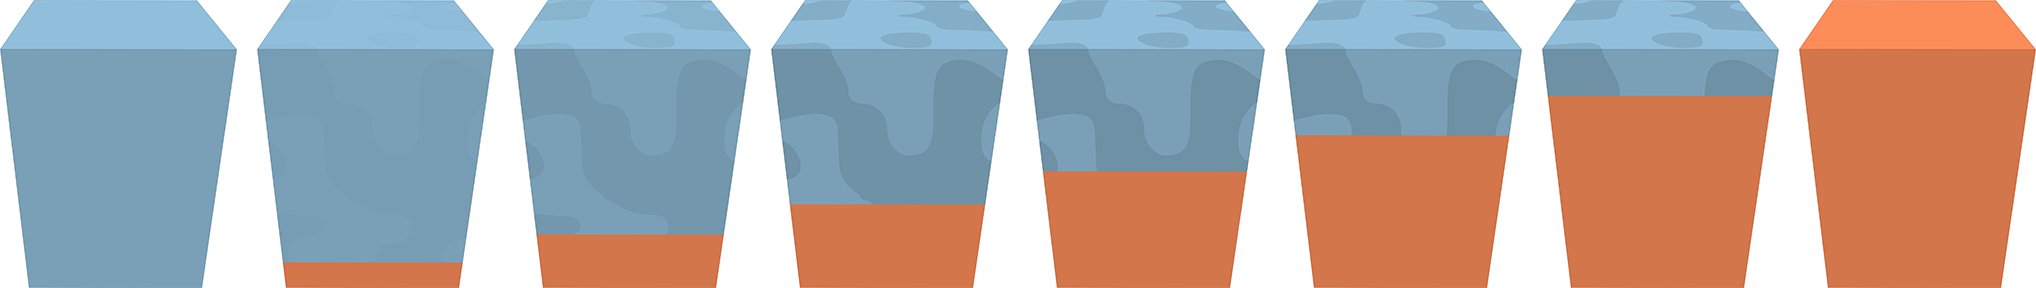
\includegraphics[width=0.85\linewidth]{figures/trans-vars-combinations-vertical-noise}}; \\
            \node[anchor=west](arrows2) {
               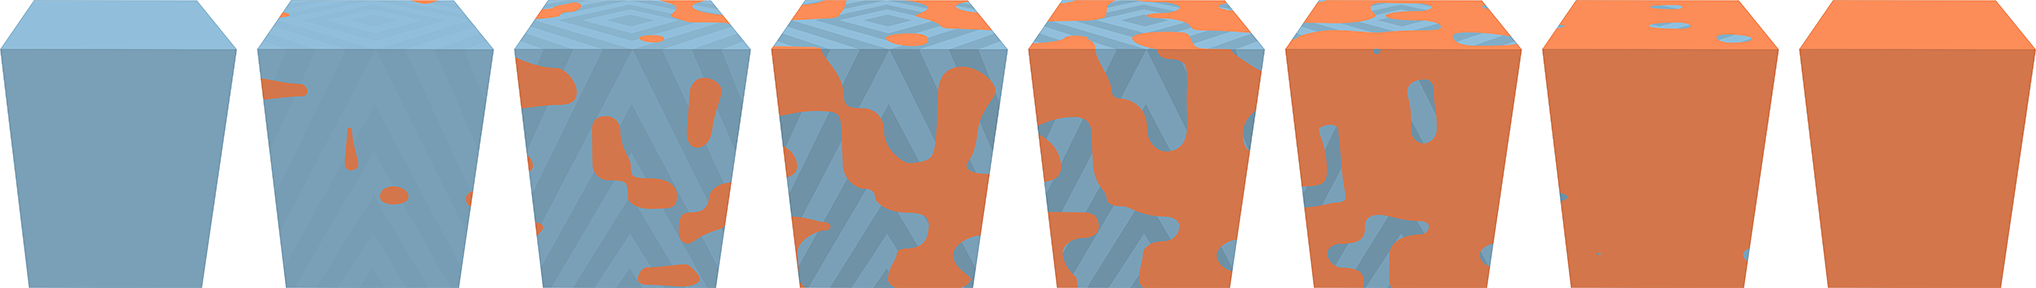
\includegraphics[width=0.85\linewidth]{figures/trans-vars-combinations-noise-arrow-full}}; \\
        };
        \spy on ($(arrows0.center)+(+0.45, +0.4)$) in node at ($(+2.0, +0.25)+(arrows0.center)$);
        \spy on ($(arrows1.center)+(+0.45, +0.4)$) in node at ($(+2.0, +0.25)+(arrows1.center)$);
        \spy on ($(arrows2.center)+(+0.45, +0.4)$) in node at ($(+2.0, +0.25)+(arrows2.center)$);
        \node[above left=1em and 1em of arrows0.north west,anchor=south east] {$t = $};
        \node[above=1em of arrows0.north west,anchor=south west] (zero) {0};
        \node[above=1em of arrows0.north east,anchor=south east] (one) {1};
        \draw[very thin,|-latex,shorten <= 1em,shorten >= 1em] (zero) -- (one);
    \end{tikzpicture}
    \caption{Combination of two procedural patterns. The dominant pattern is supported by a secondary pattern placed only on the parts representing either the former (as can be seen here) or the upcoming value. }
    \label{fig:trans-vars-combinations}
\end{figure}

\paragraph{Candidates for Secondary Use.}
Technically, the secondary pattern is not limited by the choice of the main pattern.
However, we suggest using a different, distinct pattern to the primary one, ideally one with a uniform distribution of colors.
Combining both approaches ensures that the pattern is (1) distinguishable from the main pattern and (2) visible without regard to the current transition state.
In \autoref{fig:trans-vars-combinations}, examples using the Squares pattern, the Noise pattern, and the Arrow (full) pattern as secondary pattern are shown.

\paragraph{Parameterization of Secondary Pattern.}
The secondary pattern is derived for a static progress value $\lambda = \nicefrac{1}{2}$ and applied using a blending of the base color and a darker shade.
This way, the pattern occupies half the area of the applied surface.
Regarding the choice of the applied surface, we propose to use the surface that encodes the former color to superimpose the second pattern.
The advantage of this is that the secondary pattern is only exposed (decreasingly) to the end of the transition, as the surface of the former color will vanish during the transition.
Also, the secondary pattern should not be visible at the transition's beginning but should gradually fade in.
Otherwise, the secondary pattern would appear abruptly at the beginning of a transition.

\subsection{Transition Across Multiple Visual Variables}

The proposed procedural patterns allow two states of color on a cuboid's lateral and top surfaces.
However, additional visual variables are usually used with a treemap, especially a 2.5D treemap.
For example, the node weight is mapped to the footprint area, and another attribute is mapped to height~(\autoref{fig:complex-examples}).
With these additional mappings, a transition should include the changes among all mapped visual variables~(\autoref{fig:color-and-height-change}).
Especially for the height mapping, we see visual interference with most of the proposed patterns that come into play when an animated transition is presented to the user.
Further, some patterns visually encode a direction that can be used to encode the direction of change of other visual variables, such as height.
An example pattern for this is the Arrow pattern.

\begin{figure}[tb] %
    \begin{tikzpicture}[figNS, spy using outlines = {style = spyRC, darkgray, magnification = 3.0, width = 24mm, height = 20mm}]
        \node[figRC, anchor = east](fig0) at (0,0)
            {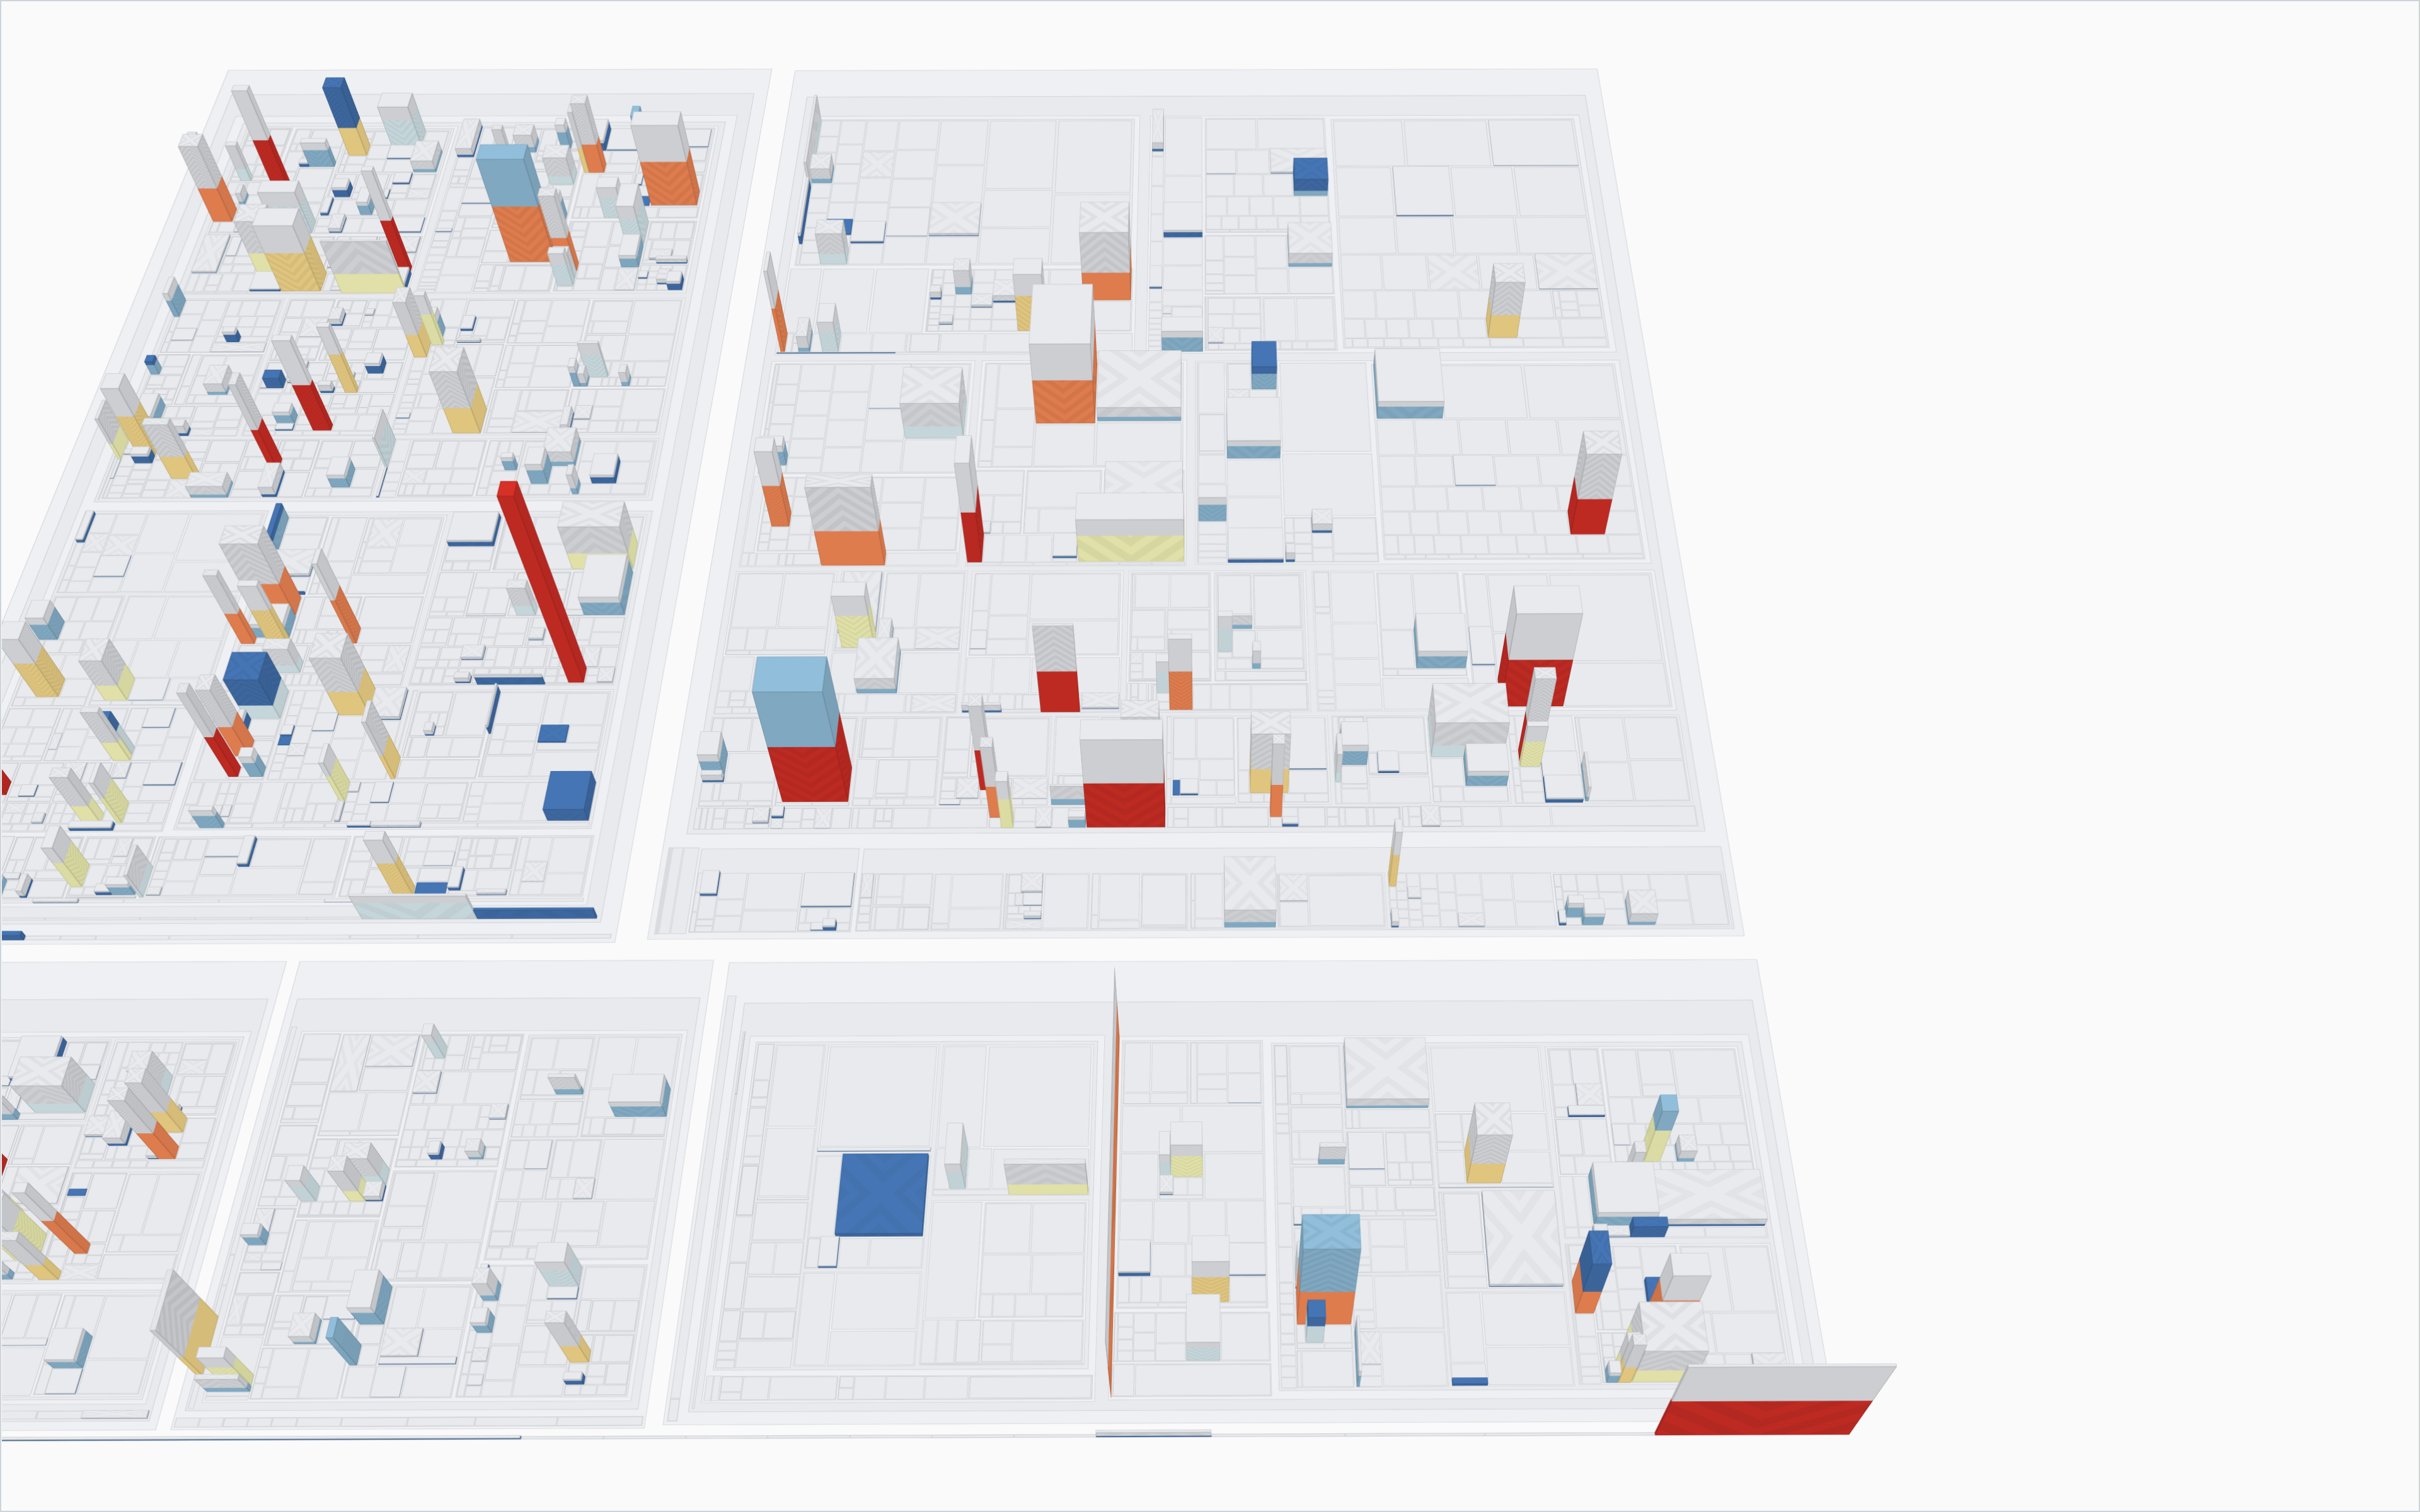
\includegraphics[width = 0.6\dimexpr(\linewidth-1.0\pfull), trim = 2 2 1040 2, clip]{figures/medium-map}};
        \node[figRC, anchor = west](fig1) at ([xshift = \pfull] fig0.east) 
            {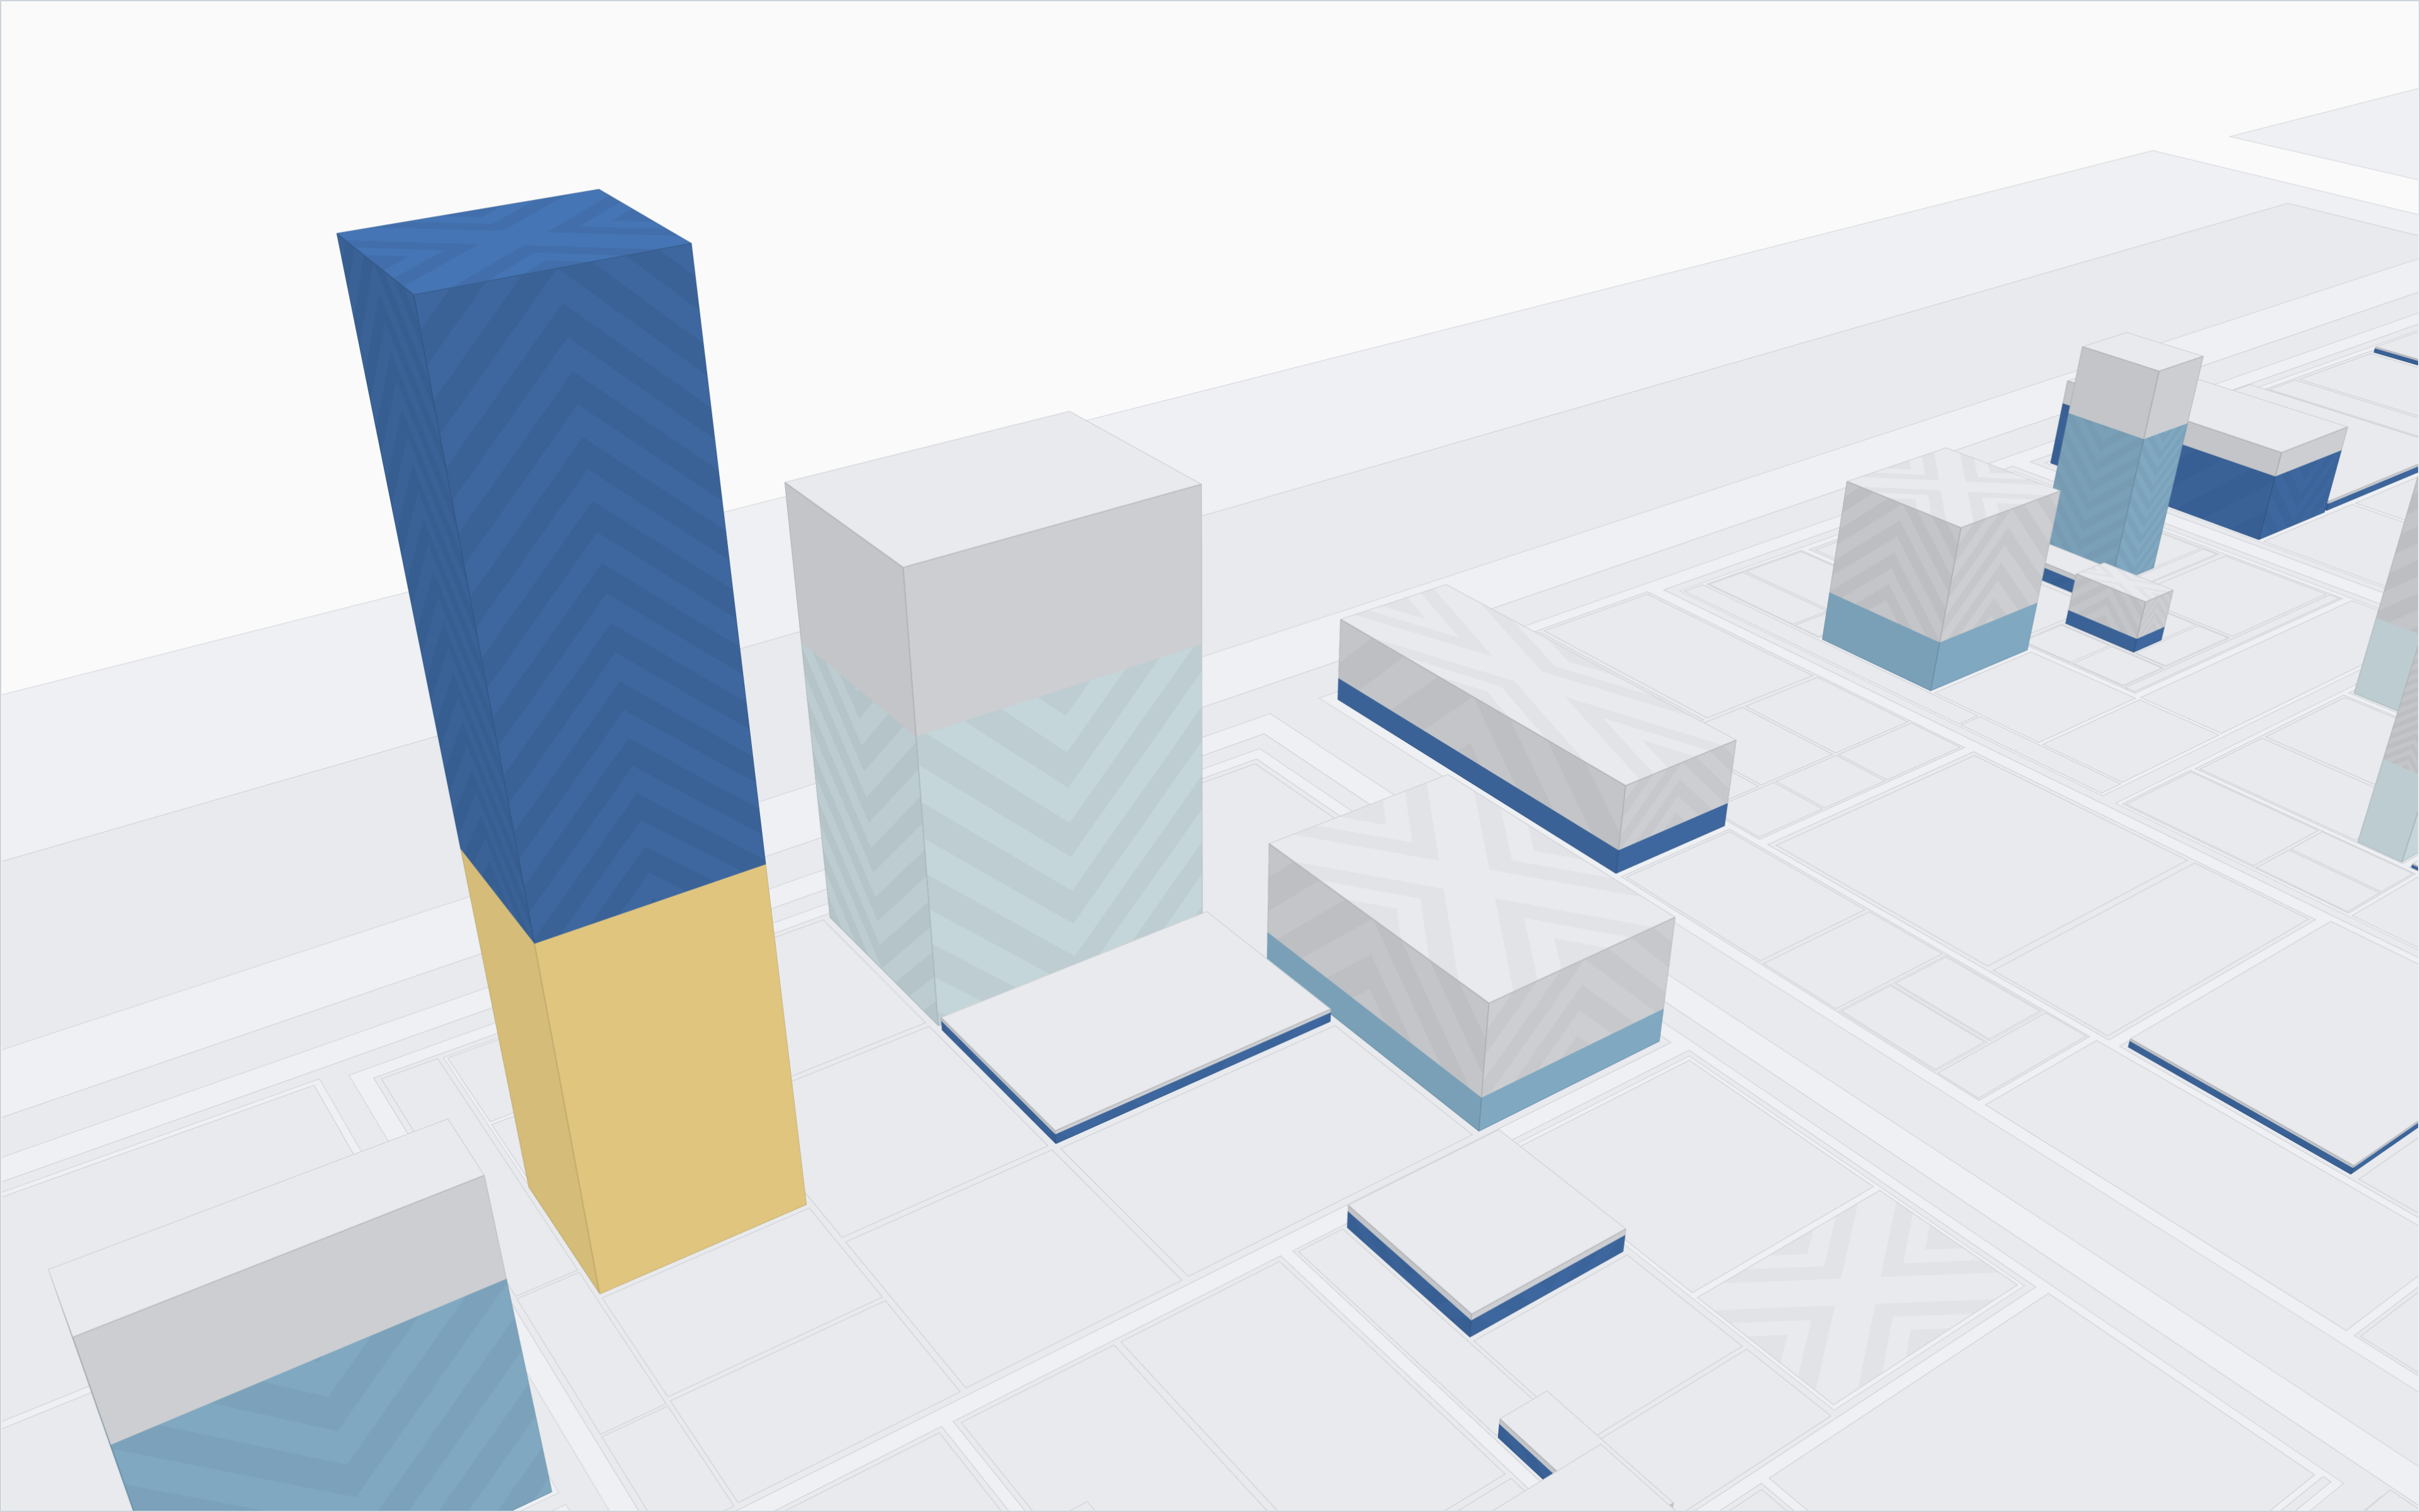
\includegraphics[width = 0.4\dimexpr(\linewidth-1.0\pfull), trim = 334 2 1640 2, clip]{figures/zoom-in-medium}};
        \node[below left = 0 of fig0, labelSW](lab0){(a)};
        \node[below left = 0 of fig1, labelSW](lab1){(b)};
        \spy on ($(fig0.center)+(-20mm, +25mm)$) in node at ($(fig0.north)+(+21mm,-12mm)$);
    \end{tikzpicture}
    \caption{%
        A software map within the middle of an animated transition of two revisions of data (a) mapped to height and color.
        For change display, the Pillar pattern is used with the Arrow (full) pattern as the secondary pattern.
        The detail view (b) shows two different changes. First, one can see that the left cuboid is growing, and its color is changing from blue to yellow. Second, the right cuboid is shrinking to zero, while the color it changes to is only used for deleted or irrelevant nodes.
    }
    \label{fig:complex-examples}
\end{figure}

\begin{figure}[tb]
    \begin{tikzpicture}[spy using outlines={white, rectangle, magnification=2.5, size=32, connect spies, every spy on node/.append style={line width=1.0pt}},inner sep=0pt, outer sep=0pt]
        \matrix[column sep=1em, row sep=1.5em] {
            \node[anchor=west](arrows0) {
                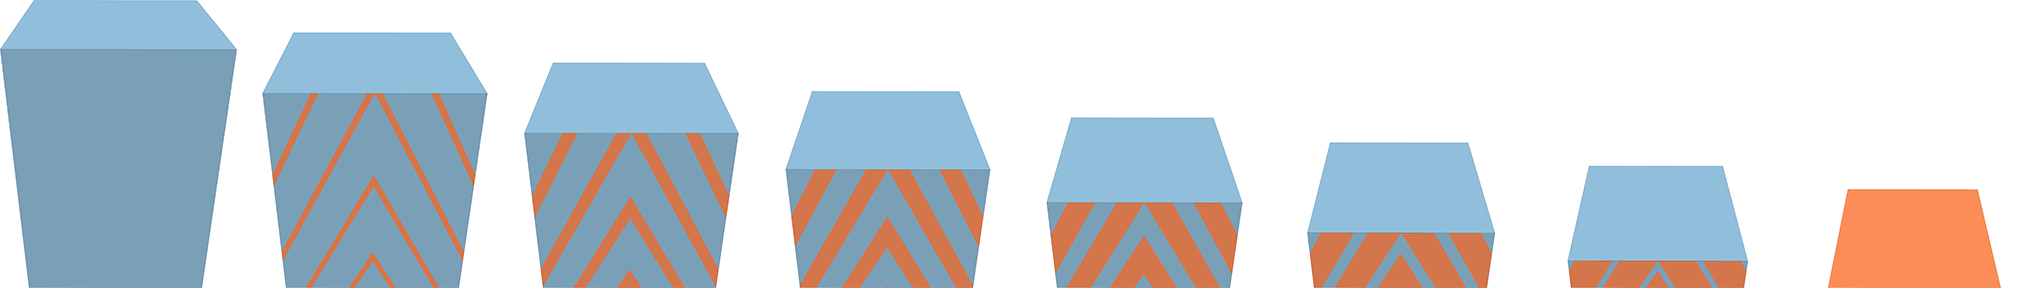
\includegraphics[width=0.85\linewidth]{figures/color-and-height-change-arrows}}; \\
            \node[anchor=west](arrows1) {
                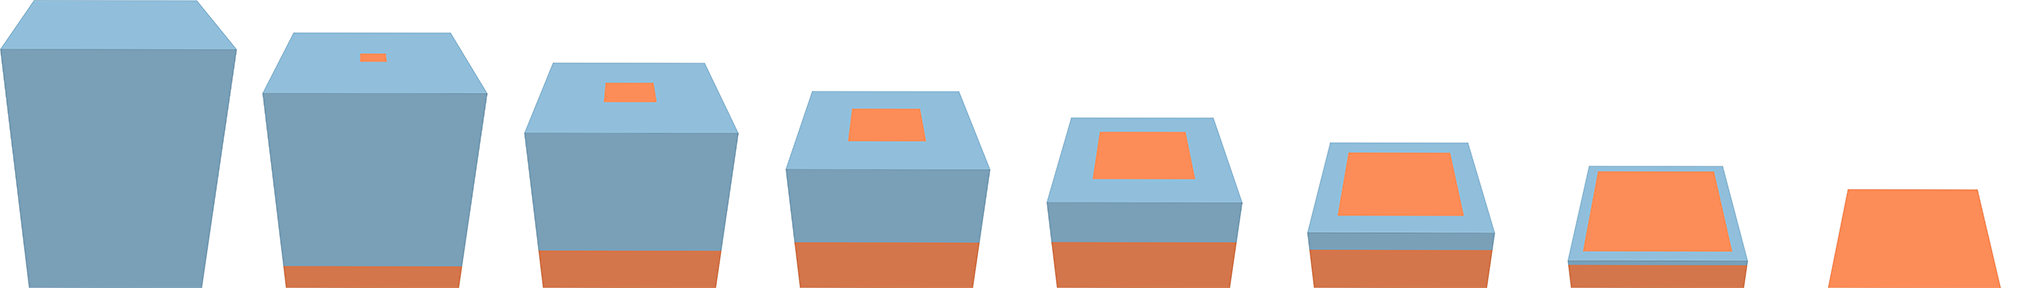
\includegraphics[width=0.85\linewidth]{figures/color-and-height-change-pyramid}}; \\
        };
        \node[above left=1em and 1em of arrows0.north west,anchor=south east] {$t = $};
        \node[above=1em of arrows0.north west,anchor=south west] (zero) {0};
        \node[above=1em of arrows0.north east,anchor=south east] (one) {1};
        \draw[very thin,|-latex,shorten <= 1em,shorten >= 1em] (zero) -- (one);
    \end{tikzpicture}
    \caption{An example of two patterns---Arrows (top) and Pyramid (bottom)---that are used to depict the simultaneous increase in color and decrease in height.}
    \label{fig:color-and-height-change}
\end{figure}

\subsection{Transitions and Animations}
So far, we have considered isolated transitions from one color to another for a single node. However, we further consider using animations and animation control to display multiple changes over a whole treemap and multiple snapshots of data.

\paragraph{Transition.}
A transition describes a change from a node's state or mapped value to another.
Thereby, a transition will not encode time or duration but only progress.
The required parameter for such a transition is its progress control $t \in [0, 1]$ where $0$ is used at the start and $1$ at the end of a transition.
This control value $t$ is then mapped to the pattern progress value $\lambda$.
In our case, we use the identity mapping $\lambda = t$, but this can be fine-tuned using other mappings as well.
Next to easing functions for aesthetic and user-experience purposes~\citep{Thomas81}, this mapping can be used to account for human perception of area ratios.

\paragraph{Animation.}
We use animation as the continuous progression over multiple states of a dataset using transitions.
More important, it is linked to the concept of time and duration.
The animation between two points in time, e.g., two subsequent revisions for software system data, can range from running all transitions for every node and every visual variable in parallel to a strict sequence.
The number of changes between two dataset states severely limits the first approach's usability.
If there are many changes or if the changes are highly scattered, a user will only be able to grasp individual changes during an animation.
The number of simultaneous transitions can be controlled with explicit management of individual transitions. For example, similar changes can be grouped, e.g., due to the same semantics or proximity within the treemap, and different changes can be ordered one after the other.
The explicit management is implemented by different starting points and transition durations for each node.
We apply different constraints to the configurations of an animation:
\begin{itemize}
    \item separate animations from different visual variables, e.g., area, height, and color,
    \item order decreases in values before increases in values, and
    \item separate animations based on proximity in the treemap.
\end{itemize}%
A configured animation from one state of a dataset to another can be handled as follows: a virtual, global time advances, and for each time-step, the per-node transition control values are updated, and the treemap is redrawn. 
This process ends as soon all transition are completed.

\section{Evaluation}
\label{sec:evaluation}
We evaluate the transition-aware patterns by applying them to software system data and a comparison of characteristics of the patterns.
The prototypical implementation is written in TypeScript and GLSL. The rendering component is based on WebGL and the rendering framework webgl-operate.
We assessed the procedural texture patterns, using them individually as well as in combination, and applied them for color change emphasis, including height and weight changes on small and large real-world datasets.
For these we used (1) an open-source project and (2) an internal, larger software project.
The results indicate the technical feasibility of the patterns, animation system, and rendering approach. However, they serve only as a starting point for much-needed user studies regarding readability of change~\citep{fiedler2020-treemapevaluation}.

\subsection{Implementation}
\label{sec:implementation}
Our prototype is an extension of a WebGL-based visualization system for large-scale 2D and 2.5D treemaps by a dual-state implementation.
We use the concept of a union tree to represent two states---a former and a latter state---of a tree-structured dataset within the visualization system~\citep{tu2007-changes}.
The system supports area, height, and color mapping as visual variables.
Specific for our prototype, we added an animation controller, adapted the geometry representation, and added pattern computation to the rendering of the cuboids.

\paragraph{Animation Controller.}
For the animation in general, we had to redesign large parts of our visualization and rendering implementation.
We composed the handling of animations and transitions to a system that manages all temporal animations, controlling the time-dependent transition values and the individual per-node transition states~(\autoref{fig:memorylayout}).
Our prototype allows for independent, simultaneous transitions per node for every mapped data attribute.
The procedural patterns are implemented as temporal visual variables, mapping a 3-tuple (a value per state and transition progress) to color.
An animation of weight and height mappings is implemented similarly.
The latter allows for ordering and masking of transitions based on (1) transition type, (2) user-defined and node-associated values, (3) metadata, (4) enumeration, and more.

\paragraph{Geometry Memory Layout.}
The geometry is based on the concept of attributed vertex clouds: Although the geometry of a cuboid has multiple vertices and corresponding polygon mesh as volatile geometry, the data for attribute mapping is represented once in GPU memory~\citep{scheibel2017-attributedvertexclouds}.
We extended this memory layout to include area, height, and color values for both the former and the latter state~(\autoref{fig:memorylayout}).
The rendering pipeline can compute a node's corresponding position, extent, and procedural texture pattern based on the per-node progress value.

\begin{figure}[tb]
    \centering
    \newlength{\blockheight}
    \setlength{\blockheight}{1.8\baselineskip}
    \tiny\ttfamily
    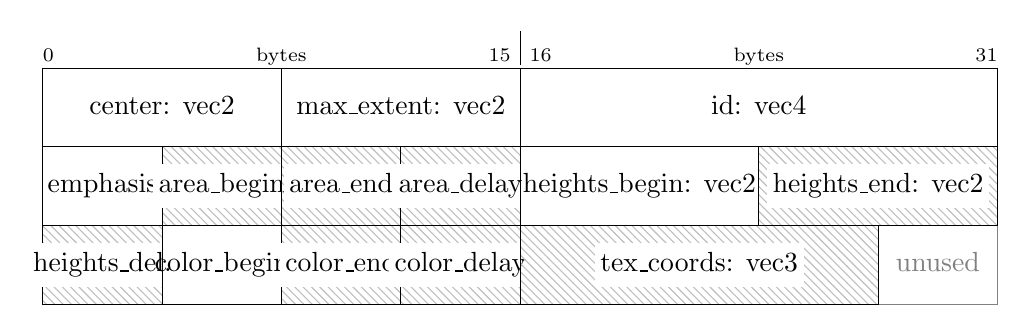
\begin{tikzpicture}[inner sep=0pt, outer sep=0pt]
        \draw[black!50!white] (0.875\linewidth, 0\blockheight) rectangle (1.000\linewidth, 1\blockheight) node[pos=0.5] (unused)     { \strut unused };
        \draw[black] (0.000\linewidth, 2\blockheight) rectangle (0.250\linewidth, 3\blockheight) node[pos=0.5] (center)          { \strut center: vec2 };
        \draw[black] (0.250\linewidth, 2\blockheight) rectangle (0.500\linewidth, 3\blockheight) node[pos=0.5] (max-extent)      { \strut max\_extent: vec2 };
        \draw[black] (0.500\linewidth, 2\blockheight) rectangle (1.000\linewidth, 3\blockheight) node[pos=0.5] (id)              { \strut id: vec4 };
        \draw[black] (0.000\linewidth, 1\blockheight) rectangle (0.125\linewidth, 2\blockheight) node[pos=0.5] (emphasis)        { \strut emphasis };
        \draw[black,pattern=north west lines, pattern color=lightgray] (0.125\linewidth, 1\blockheight) rectangle (0.250\linewidth, 2\blockheight) node[pos=0.5,fill=white,inner sep=2pt] (area-begin)      { \strut area\_begin };
        \draw[black,pattern=north west lines, pattern color=lightgray] (0.250\linewidth, 1\blockheight) rectangle (0.375\linewidth, 2\blockheight) node[pos=0.5,fill=white,inner sep=2pt] (area-end)        { \strut area\_end };
        \draw[black,pattern=north west lines, pattern color=lightgray] (0.375\linewidth, 1\blockheight) rectangle (0.500\linewidth, 2\blockheight) node[pos=0.5,fill=white,inner sep=2pt] (area-delay)      { \strut area\_delay };
        \draw[black] (0.500\linewidth, 1\blockheight) rectangle (0.750\linewidth, 2\blockheight) node[pos=0.5] (heights-begin)   { \strut heights\_begin: vec2 };
        \draw[black,pattern=north west lines, pattern color=lightgray] (0.750\linewidth, 1\blockheight) rectangle (1.000\linewidth, 2\blockheight) node[pos=0.5,fill=white,inner sep=2pt] (heights-end)     { \strut heights\_end: vec2 };
        \draw[black,pattern=north west lines, pattern color=lightgray] (0.000\linewidth, 0\blockheight) rectangle (0.125\linewidth, 1\blockheight) node[pos=0.5,fill=white,inner sep=2pt] (heights-delay) { \strut heights\_del. };
        \draw[black] (0.125\linewidth, 0\blockheight) rectangle (0.250\linewidth, 1\blockheight) node[pos=0.5] (color-begin)   { \strut color\_begin };
        \draw[black,pattern=north west lines, pattern color=lightgray] (0.250\linewidth, 0\blockheight) rectangle (0.375\linewidth, 1\blockheight) node[pos=0.5,fill=white,inner sep=2pt] (color-end)     { \strut color\_end };
        \draw[black,pattern=north west lines, pattern color=lightgray] (0.375\linewidth, 0\blockheight) rectangle (0.500\linewidth, 1\blockheight) node[pos=0.5,fill=white,inner sep=2pt] (color-delay)   { \strut color\_delay };
        \draw[black,pattern=north west lines, pattern color=lightgray] (0.500\linewidth, 0\blockheight) rectangle (0.875\linewidth, 1\blockheight) node[pos=0.5,fill=white,inner sep=2pt] (texcoords)     { \strut tex\_coords: vec3 };
        \node[anchor=south west] at (0.0\linewidth, 3\blockheight) { \scriptsize \strut 0 };
        \node[anchor=south] at (0.25\linewidth, 3\blockheight) { \scriptsize \strut bytes };
        \node[anchor=south east] at (0.49\linewidth, 3\blockheight) { \scriptsize \strut 15 };
        \draw[black,shorten <= 1pt,shorten >= 1pt] (0.5\linewidth, 3\blockheight) -- ($(0.5\linewidth, 3\blockheight) + (0cm,1.2\baselineskip)$);
        \node[anchor=south west] at (0.51\linewidth, 3\blockheight) { \scriptsize \strut 16 };
        \node[anchor=south] at (0.75\linewidth, 3\blockheight) { \scriptsize \strut bytes };
        \node[anchor=south east] at (1.0\linewidth, 3\blockheight) { \scriptsize \strut 31 };
    \end{tikzpicture}
    \caption{
        Illustration of the memory layout of the per-cuboid data. The cell's width corresponds to the memory consumption; the base width corresponds to one float, i.e., $4$\,bytes, and multiples of two, three, and four corresponds to the vector formats vec2, vec3, and vec4, respectively. The memory representation thus consumes 92 bytes per cuboid.
        This per-cuboid data allows representing both a former state and a latter state for area mapping, height mapping, and color mapping. Further, each mapping has an individual delay value for each cuboid to allow fine-grained animation control. The \emph{emphasis} affects the kind of visual emphasis on the node, e.g., outlines or highlighting fill color.
        The pattern indicates the per-cuboid data that was added to support animated transitions.
        The per-cuboid data for a static display consumes 48 bytes.}
    \label{fig:memorylayout}
\end{figure}

\begin{figure}[tb]
    \centering%
    \pgfplotstableread[col sep=comma,]{measurements/performance.csv}\datatable%
    \pgfplotstablefilter[implementation equals {basic}]{\datatable}{\datatableB}%
    \pgfplotstablefilter[implementation equals {dualstate}]{\datatable}{\datatableDS}%
    \pgfplotstablefilter[implementation equals {dualstate-animated}]{\datatable}{\datatableDSA}%
    \begin{tikzpicture}[outer sep=0pt]%
        \begin{axis}[
        	compat=newest,
        	name=traversal,
        	ybar=5pt,
        	scaled y ticks=false,
        	width=0.6\columnwidth,
        	height=14\baselineskip,
        	enlarge x limits=0.6,
        	bar width=8.0pt,
        	ylabel=\footnotesize{Average frame time in ms},
        	xlabel=\footnotesize{Treemap Size},
        	ymajorgrids,
        	major grid style={draw=white},
        	tick label style={font=\scriptsize},
        	yticklabel style={
        		/pgf/number format/fixed,
        		/pgf/number format/precision=1
        	},
        	xticklabel style={
        	    align=center,
    	    },
        	axis x line*=bottom,
        	axis y line*=left,
        	ytick align=outside,
        	xtick=data,
        	xticklabels={{Small Treemap\\($\approx$3\,800 nodes)}, {Large Treemap\\($\approx$450\,000 nodes)}},
        	ymin=0.0,
        	ymax=40.0,
        	point meta=rawy,
        	nodes near coords,
        	every node near coord/.append style={rotate=90, anchor=west, font=\scriptsize,/pgf/number format/.cd, precision=1, fixed,1000 sep={\,}},
	        nodes near coords align={vertical},
    	]
        	\addplot[white,very thin,fill=plots-1,text=black] table[y={frametime},x expr=\coordindex]{\datatableB};
        	\addplot[white,very thin,fill=plots-2,text=black] table[y={frametime},x expr=\coordindex]{\datatableDS};
        	\addplot[white,very thin,fill=plots-3,text=black] table[y={frametime},x expr=\coordindex]{\datatableDSA};
    	\end{axis}
    	\begin{axis}[
        	compat=newest,
        	name=fps,
        	width=0.6\columnwidth,
        	height=14\baselineskip,
        	hide axis,
        	xmin=-0.6,
        	xmax=1.6,
        	ymin=0.0,
        	ymax=40.0,
    	]
        	\addplot[dashed,white!60!black] {16.67};
        	\node[right,white!60!black] at (axis cs: -0.6,19.00) {\scriptsize 60\,FPS};
        	\addplot[dashed,white!60!black] {33.33};
        	\node[right,white!60!black] at (axis cs: -0.6,35.00) {\scriptsize 30\,FPS};
    	\end{axis}
    	\begin{axis}[
        	name=traversal_legend,
        	compat=1.3,
        	at={($(traversal.north east)+(0.0cm,0.0cm)$)},
        	hide axis,
        	bar width=0pt,
        	ticks=none,
        	legend style={
        		at={(0.0,0.0)},
        		anchor=north west,
        		draw=none,
        		legend cell align=left,
        	},
        	legend image code/.code={%
        		\draw (0.0cm,-0.05cm) rectangle (0.4cm,0.15cm);
        	},
        	text height=1.1ex,
        	height=2cm,
        	ymin=0.0,
        	ymax=1.0,
        	xmin=0.0,
        	xmax=1.0
        ]
        	\addplot[draw=none,white,very thin,fill=plots-1] coordinates {(0,0)};
        	\addlegendentry{\;\scriptsize Base Implementation}
        	\addplot[draw=none,white,very thin,fill=plots-2] coordinates {(0,0)};
        	\addlegendentry{\;\scriptsize Dual-State Implementation}
        	\addplot[draw=none,white,very thin,fill=plots-3] coordinates {(0,0)};
        	\addlegendentry{\;\scriptsize Dual-State (during Animation)}
        \end{axis}%
    \end{tikzpicture}%
    \vspace{-0.5\baselineskip}
    \caption{
        Performance analysis on a small treemap and a large treemap example based on the base implementation and the dual-state implementation, as well as an additional measure for the dual-state implementation during an active animation. The system for the measurements was a Ryzen 5 1600X CPU with 16GB RAM and an Nvidia GTX 1060 GPU with 6GB VRAM. The target resolution for rendering was FullHD (1080$\times$1920 pixels). Each measure is the average of 32\,000 frame renderings.
    }
    \label{fig:performanceanalysis}
\end{figure}

\paragraph{Pattern Computation.}
The implementation uses fragment shaders and consists of the actual pattern computation and a blending with the other aspects of the shading~(\autoref{listing:fragment_color_blending}, \autoref{listing:vertical_pattern_implementation}). 
Implementing the patterns themselves was straightforward and imposed no significant impact on rendering performance (runs on mobile devices for large treemaps up to 100\,000 nodes).
For desktop machines, the performance impact was around 30\% compared to the base implementation~(\autoref{fig:performanceanalysis}.
The patterns are implemented using \emph{signed distance functions}~\citep{Vivo} and fragment shaders.
The patterns differ mainly in appearance, granularity, and intended surfaces, but they share a constant run-time overhead.

\begin{lstlisting}[language = glsl, label = listing:fragment_color_blending, caption = {%
    Excerpt of the GLSL fragment shader for shading treemap cuboids with patterns of the proposed pattern catalog. Secondary patterns are considered as well. The actual implementation of a pattern resides in \texttt{calculateColorDistance}, which is shown in \autoref{listing:vertical_pattern_implementation}.}]
struct PatternConfig {
    int mode; // type of pattern, e.g., pillar
    float progress; // node-local progress value
};

struct PatternData {
    int face; // the current axis-oriented face of a cuboid
    float nodeCountSqrt; // pattern scale factor
    vec2 texCoord2D; // face-local 2D coordinates
    vec3 texCoord3D; // cuboid-local 3D coordinates
    vec3 uv; // pattern-adjusted local 3D coordinates
    vec4 worldPos; // treemap-global 3D coordinates
    float relativeHeight; // relative height of cuboid
    float absoluteHeight; // absolute height of cuboid
};

PatternData patternData = PatternData(
    u_face, u_nodeCountSqrt, v_texCoord2D, v_texCoord3D,
    v_uv, v_worldPos, v_relativeHeight, v_absoluteHeight
);
 
PatternConfig diffPatternConfig = PatternConfig(
    u_diffPatternMode, 0.5
);

PatternConfig colorConfig = PatternConfig(
    u_colorMode, v_colorProgress
);

// returns distance to border between base color and target color.
//  <  0 represents base color
//  >= 0 represents target color
float calculateColorDistance(in PatternData data, in PatternConfig config);

void main() {
    // ...
    float baseColorDistance = 
        calculateColorDistance(patternData, diffPatternConfig);
    float baseColorDecider = smoothstep(0.0, 0.5, v_colorProgress) 
        * step(0.0, baseColorDistance);
    float colorDistance = calculateColorDistance(patternData, colorConfig);
    float colorDecider = step(0.0, colorDistance);
    vec4 colorBegin = 
        mix(v_baseColorBegin, v_patternColorBegin, baseColorDecider);
    fragColor = mix(baseColorBegin, v_baseColorEnd, colorDecider);
}
\end{lstlisting}

\begin{lstlisting}[language = glsl, label = listing:vertical_pattern_implementation, caption = {%
    Example implementation of the \emph{vertical} pattern in GLSL. \autoref{listing:fragment_color_blending} contains the definitions for \texttt{PatternData} and \texttt{PatternConfig}.}]
// returns distance to border between base color and target color.
//  <  0 represents base color
//  >= 0 represents target color
float calculateColorDistance(in PatternData data, in PatternConfig config) {
    // vertical pattern
    if (config.mode == 0) {
        return config.progress - data.relativeHeight;
    }
    // ...
    
    // default
    return 0.0; // means base color
}
\end{lstlisting}

\begin{figure}[tb]
    \centering
    \begin{tikzpicture}[figNS, spy using outlines = {style = spyRC, darkgray, magnification = 2.25, size = 64}]
        \matrix[column sep=1em, row sep=0.33em] {
            \node[] (state-0) { 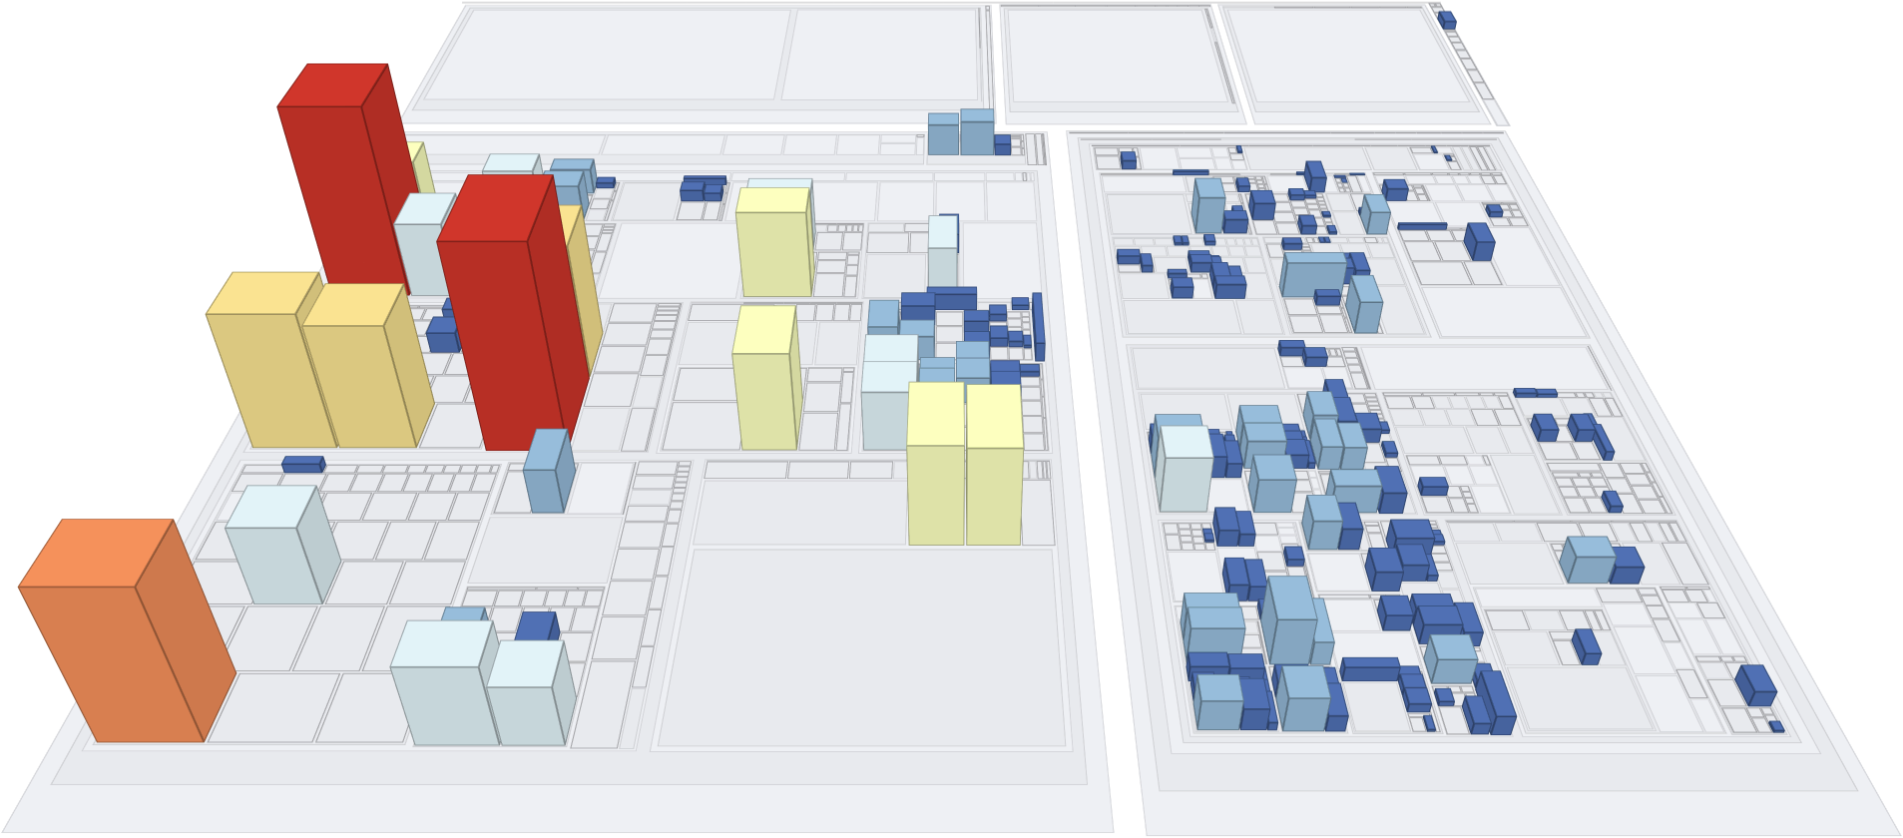
\includegraphics[width=0.48\linewidth]{figures/demo2-0.png} }; &
            \node[] (state-1) { 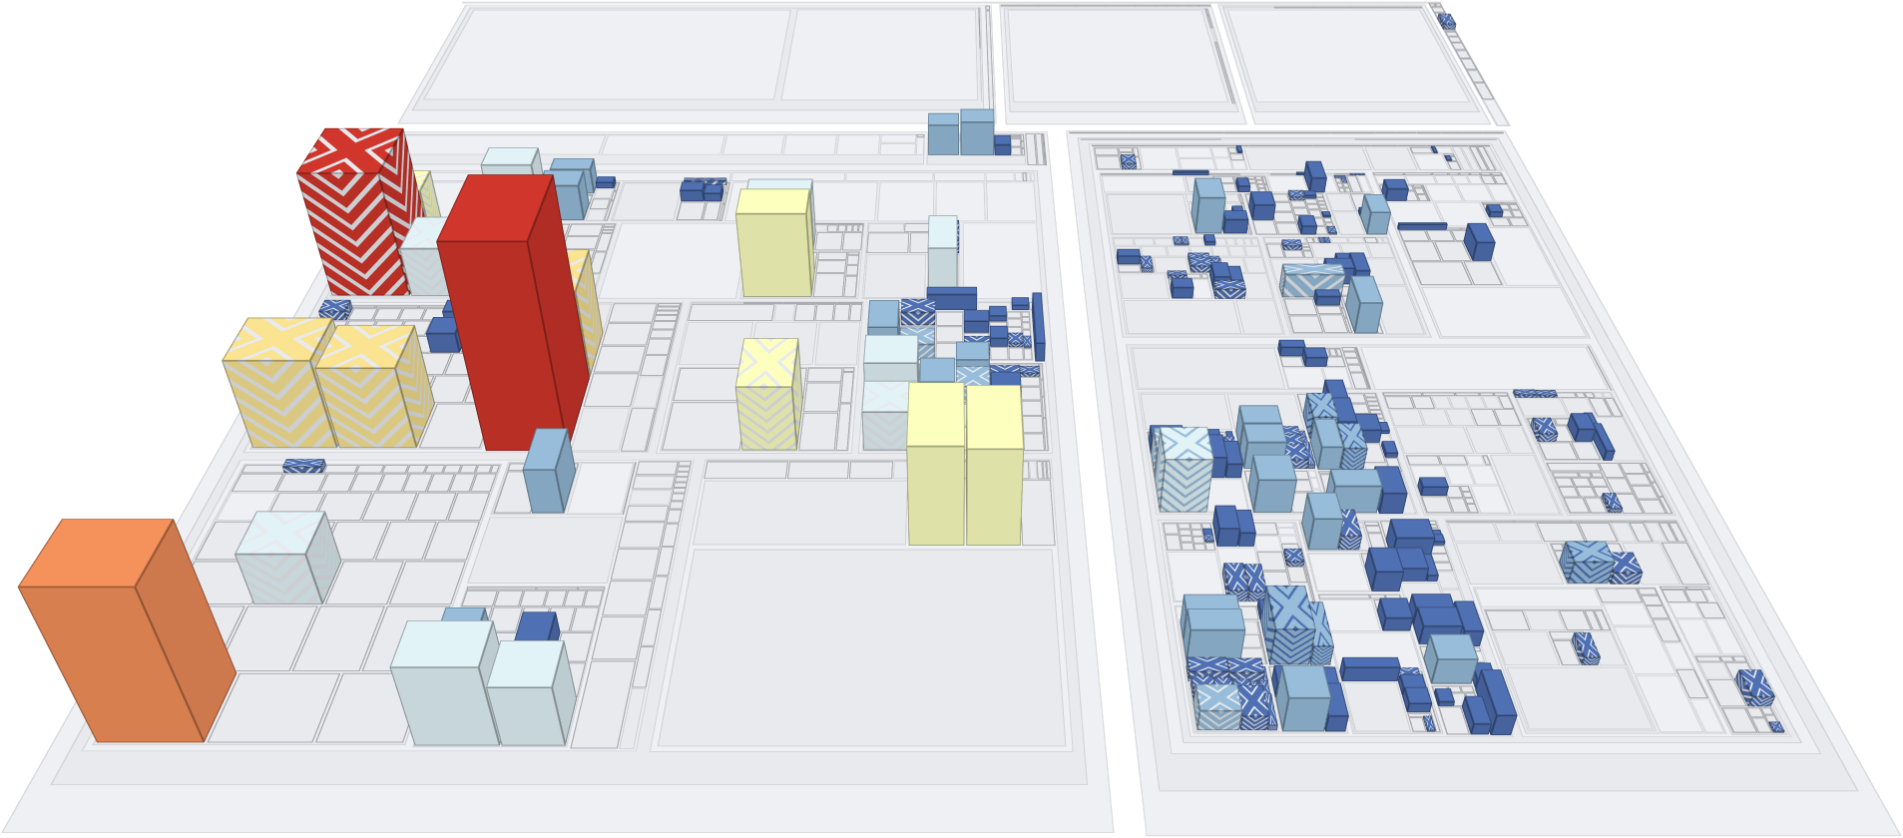
\includegraphics[width=0.48\linewidth]{figures/demo2-1.png} }; \\
            \node[] { $t = 0$ }; &
            \node[] { $t = \nicefrac{1}{3}$ }; \\
            & \\
            & \\
            & \\
            \node[] (state-2) { 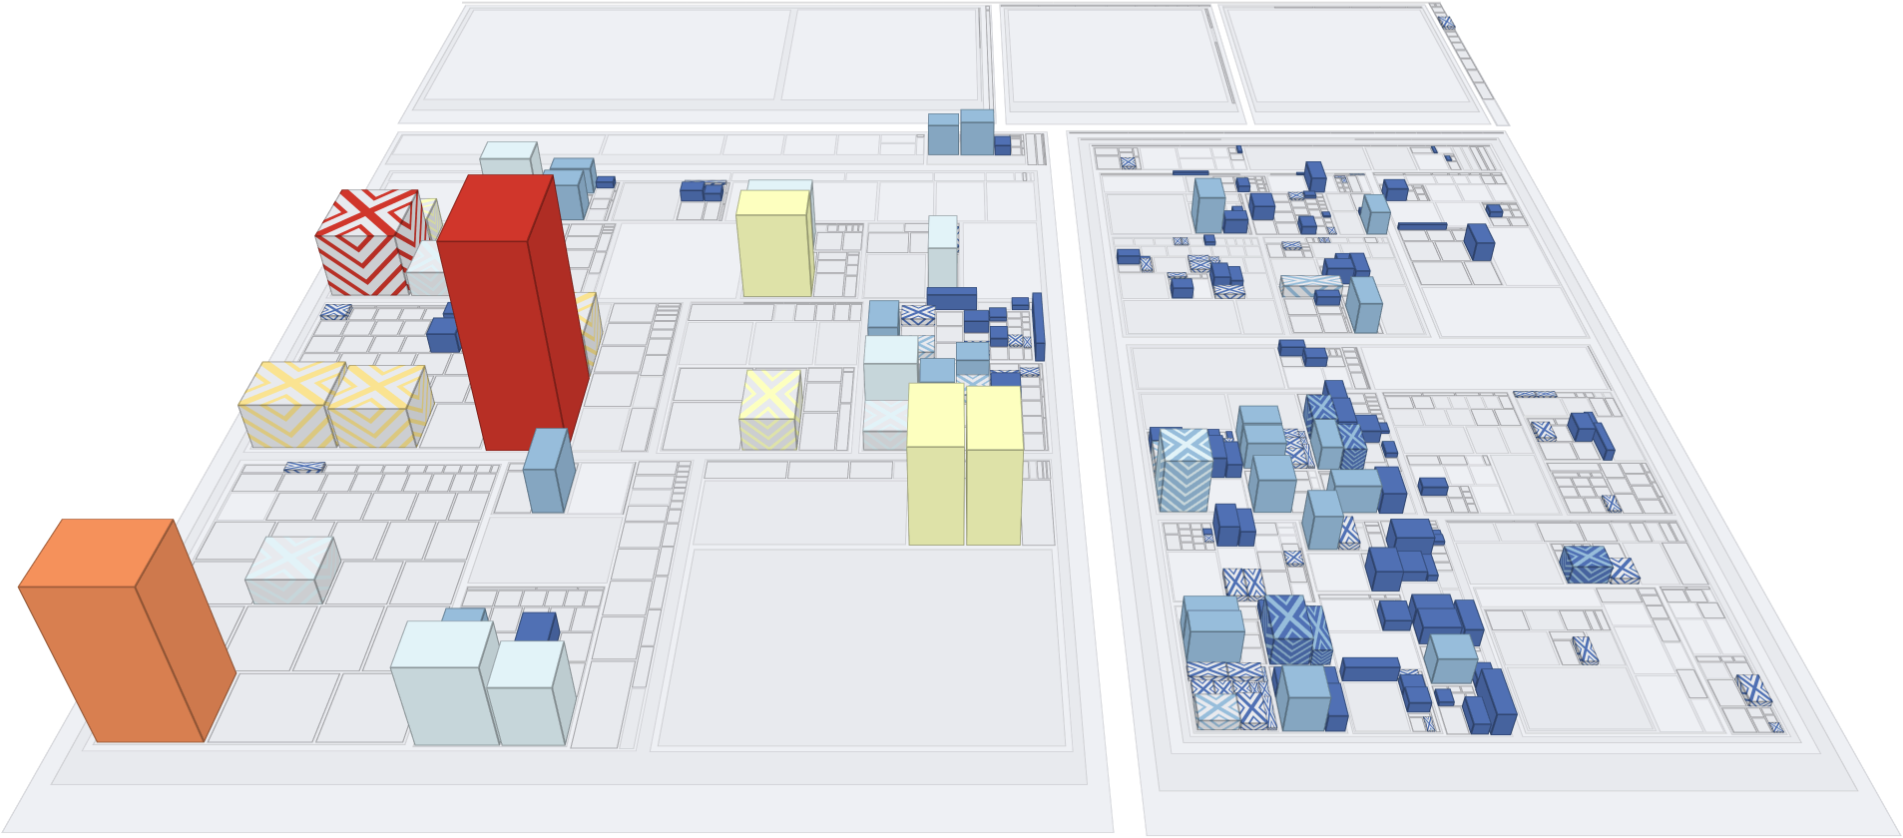
\includegraphics[width=0.48\linewidth]{figures/demo2-2.png} }; &
            \node[] (state-3) { 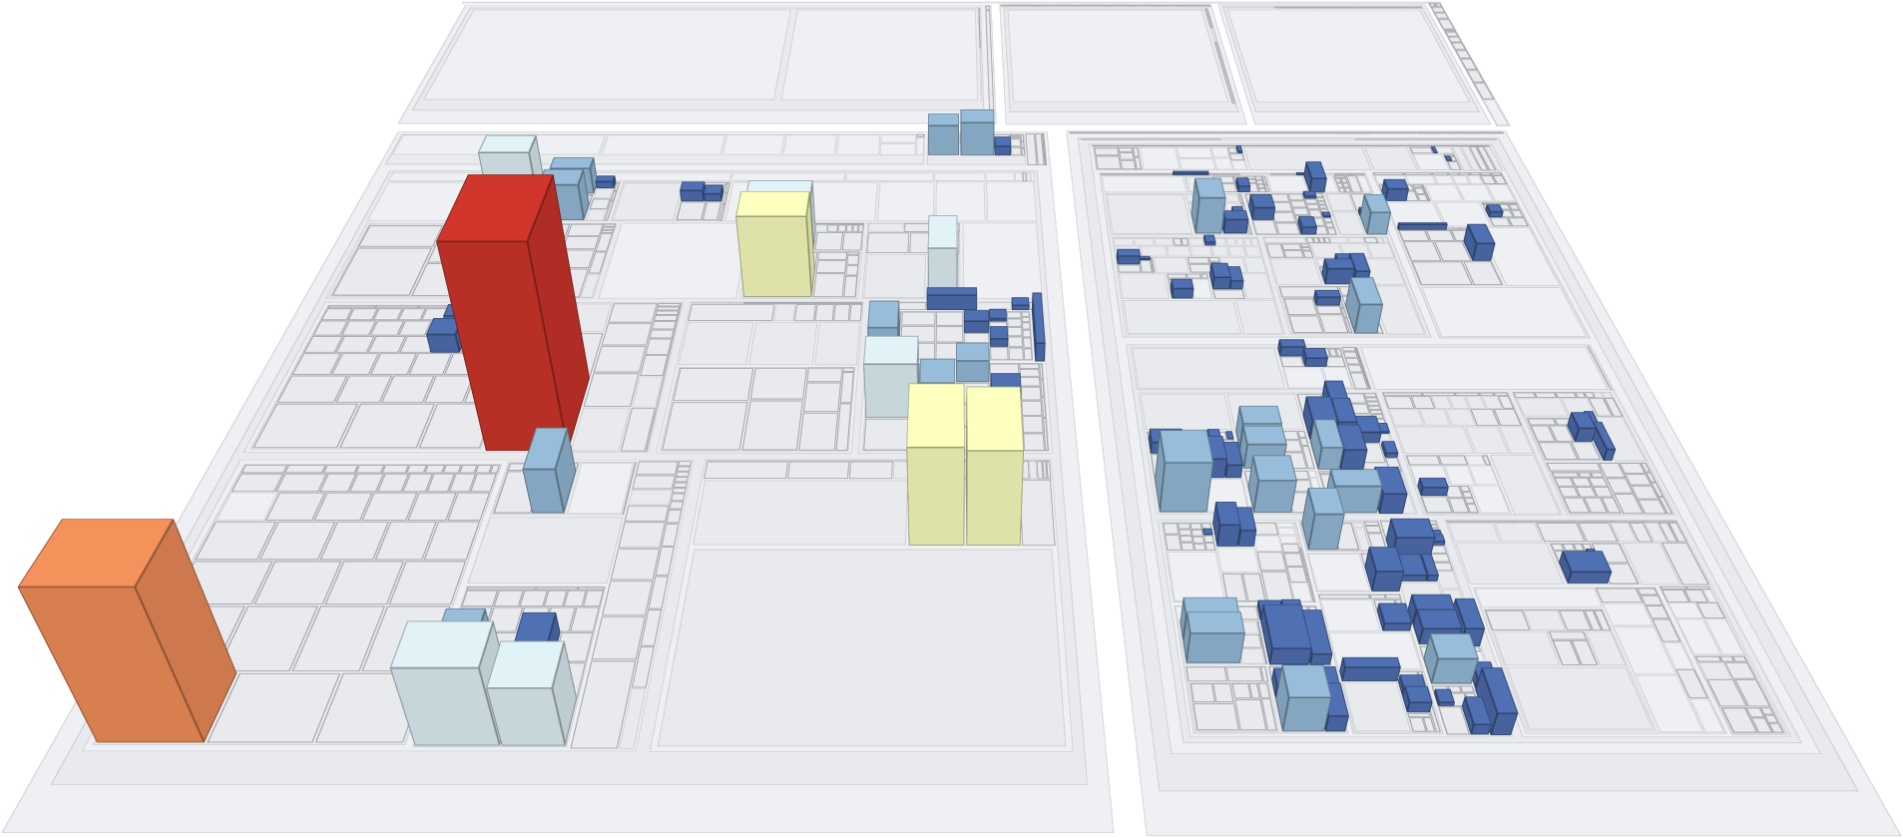
\includegraphics[width=0.48\linewidth]{figures/demo2-3.png} }; \\
            \node[] { $t = \nicefrac{2}{3}$ }; &
            \node[] { $t = 1$ }; \\
        };
        \spy on ($(state-0.center)+(-1.8, +0.65)$) in node at ($(state-0.center)+(+1.4, 0.0)$);
        \spy on ($(state-1.center)+(-1.8, +0.65)$) in node at ($(state-1.center)+(+1.4, 0.0)$);
        \spy on ($(state-2.center)+(-1.8, +0.65)$) in node at ($(state-2.center)+(+1.4, 0.0)$);
        \spy on ($(state-3.center)+(-1.8, +0.65)$) in node at ($(state-3.center)+(+1.4, 0.0)$);
    \end{tikzpicture}
    \caption{
        Four snapshots with progress values of $0$, $\nicefrac{1}{3}$, $\nicefrac{2}{3}$, and $1$ of an animated transition between the state of the software project \emph{cpplocate} from October 27, 2018, to March 2, 2019.
    }
    \label{fig:casestudy}
\end{figure}

\begin{figure}[tb] %
    \begin{tikzpicture}[figNS, spy using outlines = {style = spyRC, darkgray, magnification = 3.0, width = 24mm, height = 20mm}]
        \node[figRC, anchor = east](fig0) at (0,0)
            {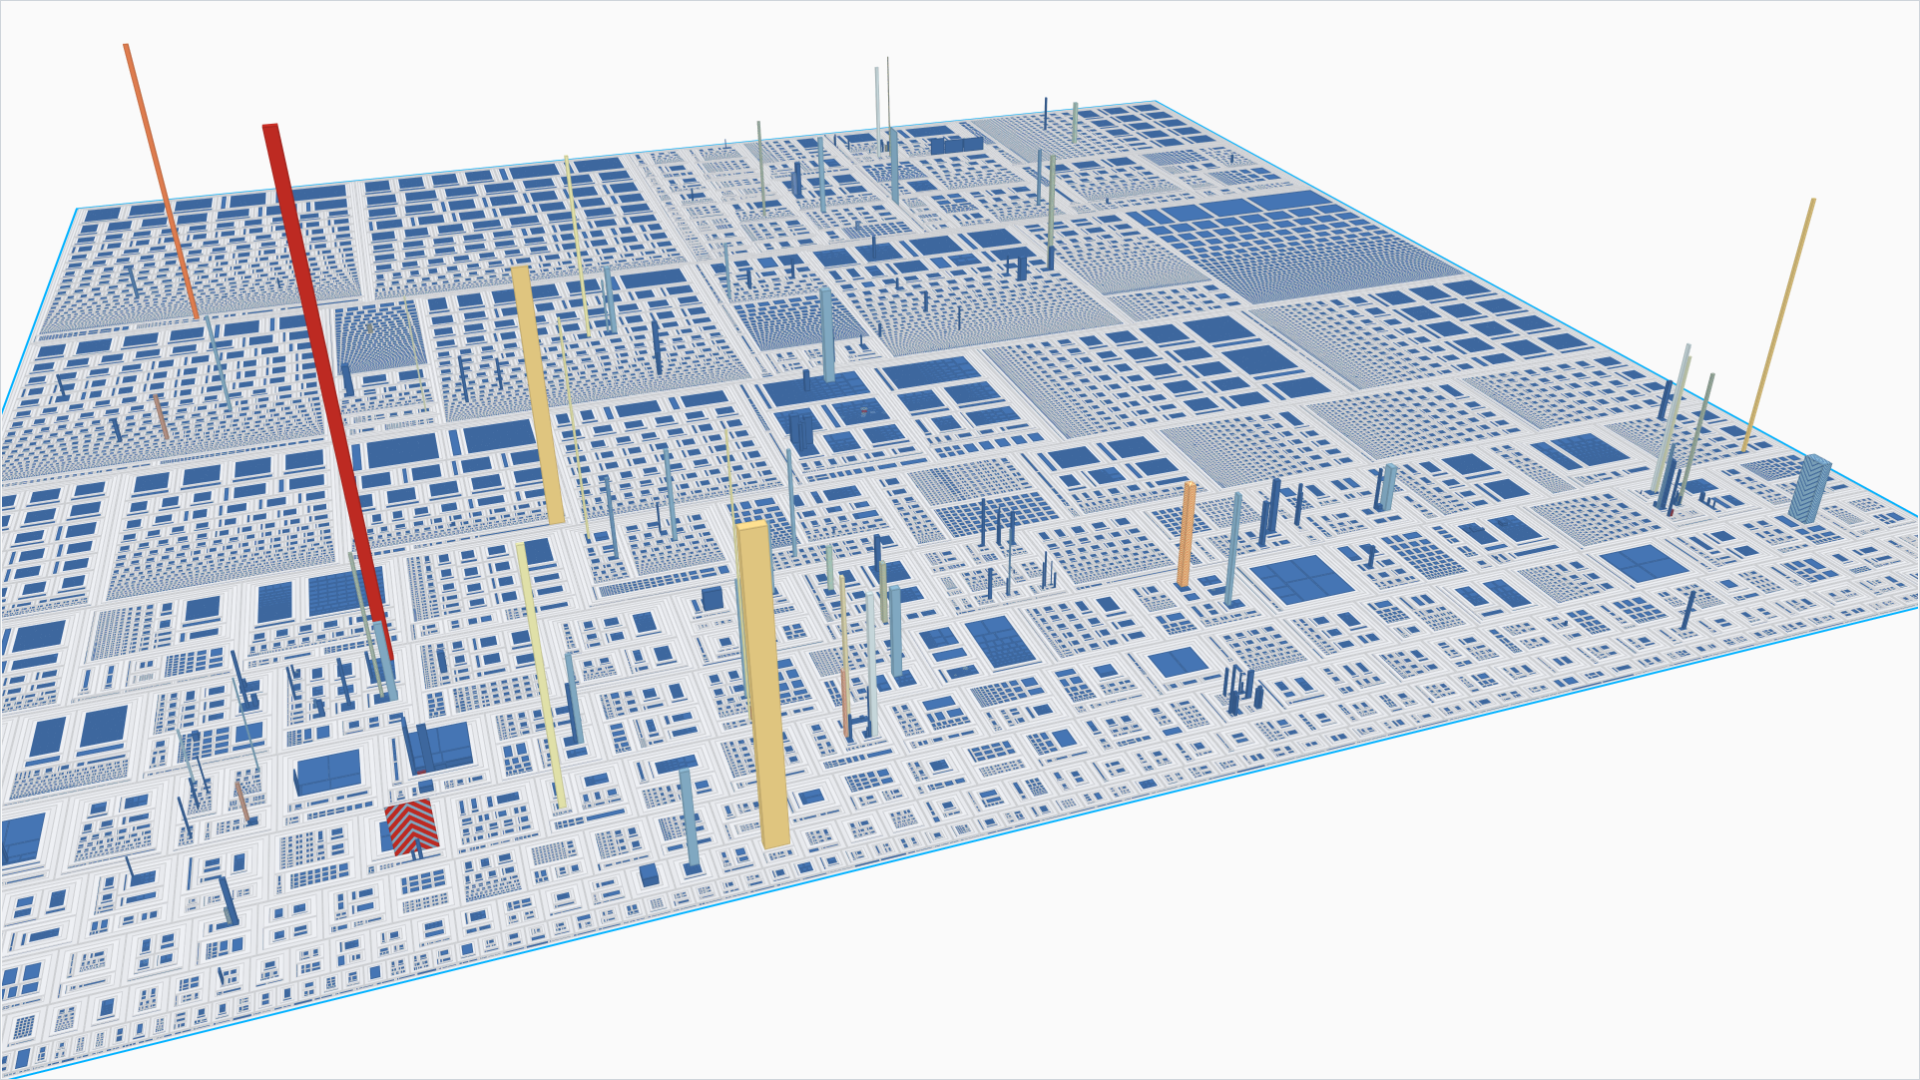
\includegraphics[width = 1.0\linewidth]{figures/large-treemap-animation.png}};
        \spy on ($(fig0.center)+(-34mm, -18mm)$) in node at ($(fig0.south east)+(-38mm,+11mm)$);
        \spy on ($(fig0.center)+(+52.5mm, +3.25mm)$) in node at ($(fig0.south east)+(-13mm,+11mm)$);
    \end{tikzpicture}
    \caption{%
        Software map of an internal software project with above 450\,000 nodes. It is displayed within the middle of an animated transition of two revisions of data.
        For change display, the \emph{Arrow} pattern is used for increasing values and an inversed \emph{Arrow} pattern is used for decreasing values. 
    }
    \label{fig:large-example}
\end{figure}

\subsection{Case Study}
Based on the software prototype, we applied the texture patterns on a software system dataset created from the structure and measured software metrics on the Open Source C++ project \emph{cpplocate}\footnote{Source code hosted on GitHub at \href{https://github.com/cginternals/cpplocate}{https://github.com/cginternals/cpplocate}, which, at the time of measurement, still included \emph{googletest} as an in-source module.}.
The source code was measured for the metrics \emph{lines of code}, \emph{nesting level}, \emph{cyclomatic complexity}, \emph{number of developers}, and \emph{change frequency}.
For this example, the former state was set to October 27, 2018, while the latter state for analysis was March 2, 2019.
The used mappings are \emph{lines of code} for area mapping, \emph{cyclomatic complexity} for height mapping, resulting in an abstract volume of implementation for the volume of the cuboid of the treemap, and the \emph{change frequency} for color mapping. 

The visualization highlights that only parts of the software system changed during this period, which is expected for software development~(\autoref{fig:casestudy}).
Further, it shows a decrease in change frequency (mapped to color), and cyclomatic complexity (mapped to height) for the source code module in focus.
The change in the color attribute could be encoded in the procedural texture pattern, while the change in the height attribute was only incidentally decreasing, too.

In comparison, we also applied the visualization to a closed-source software system dataset with above 450\,000 nodes~(\autoref{fig:large-example}).
The number of nodes results in a small screen space for average-sized nodes.
As a result, changes on small and average-sized nodes get overlooked.
Regarding run-time performance, adding the procedural texture patterns had a noticeable effect~(\autoref{fig:performanceanalysis}). The average frame time dropped below 30 frames per second but still allowed for animated transitions.

\settowidth{\largestheaderlength}{$\nabla_{\textrm{DirChange}}$}%
\begin{table}[b]
    \centering
    \renewcommand{\arraystretch}{2.0}
    \rowcolors{0}{white}{gray!10}%
    \setlength{\tabcolsep}{6pt}%
    \begin{tabularx}{1.0\linewidth}{rXcccccc|ccccc}
        \multicolumn{2}{l}{} &
        \multicolumn{6}{c|}{\textbf{Encoding -- $\nabla E$}} &
        \multicolumn{5}{c}{\textbf{Compatibility -- $\nabla C$}} \\
        \rowcolor{white}
        \multicolumn{2}{l}{\textbf{Procedural Pattern}\rott{\parbox{\largestheaderlength}{~}}} &
        \rot{\makecell[l]{\strut $\nabla_{\textrm{Monotonic}}$}} &
        \rot{\makecell[l]{\strut $\nabla_{\textrm{DirStates}}$}} &
        \rot{\makecell[l]{\strut $\nabla_{\textrm{DirChange}}$}} &
        \rot{\makecell[l]{\strut $\nabla_{\textrm{RatioLat}}$}}  &
        \rot{\makecell[l]{\strut $\nabla_{\textrm{RatioTop}}$}}  &
        $\sum_{\nabla E}$ &
        \rot{\makecell[l]{\strut $\nabla_{\textrm{IndHeight}}$}} &
        \rot{\makecell[l]{\strut $\nabla_{\textrm{IndWeight}}$}} &
        \rot{\makecell[l]{\strut $\nabla_{\textrm{TreeSize}}$}} &
        \rot{\makecell[l]{\strut $\nabla_{\textrm{Polygonal}}$}} &
        $\sum_{\nabla C}$ \\
        \midrule
        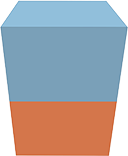
\includegraphics[height=1.9em,align=m,vshift=0.5em]{figures/vertical-50-dark-sm-alpha} & \strut%
            Pillar         & \OK & \OK & -- & \OK & --  & 3 & \PARTIAL  & \OK      & \OK & \OK & 3.5 \\
        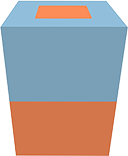
\includegraphics[height=1.9em,align=m,vshift=0.5em]{figures/pyramid-50-dark-sm-alpha}     & \strut%
            Pyramid        & \OK & \OK & -- & \OK      & \PARTIAL & 3.5 & \PARTIAL  & \OK & \OK & \PARTIAL & 3 \\
        
\includegraphics[height=1.9em,align=m,vshift=0.5em]{figures/dithering-50-dark-sm-alpha}   & \strut%
            Dithering      & \OK & --  & -- & \OK     & \OK  & 3 & \OK & \OK      & \OK & \OK & 4 \\
        
\includegraphics[height=1.9em,align=m,vshift=0.5em]{figures/arrows-50-dark-sm-alpha}      & \strut%
            Arrows         & \OK & --  & \OK & \OK & --  & 3 & \OK & \OK      & \PARTIAL & \PARTIAL & 3 \\
        
\includegraphics[height=1.9em,align=m,vshift=0.5em]{figures/arrows-full-50-dark-sm-alpha} & \strut%
            Arrows (full)  & \OK & --  & \OK & \OK      & \OK & 4 & \OK & \OK      & \PARTIAL & -- & 2.5 \\
        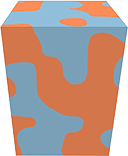
\includegraphics[height=1.9em,align=m,vshift=0.5em]{figures/noise-50-dark-sm-alpha}       & \strut%
            Noise          & \OK & --  & -- & \PARTIAL       & \PARTIAL & 2 & \OK & \OK      & \PARTIAL & \OK & 3.5 \\
        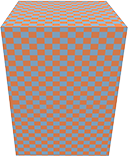
\includegraphics[height=1.9em,align=m,vshift=0.5em]{figures/quads-50-dark-sm-alpha}       & \strut%
            Squares        & \OK & --  & -- & \OK      & \OK & 3 & \OK & \OK      & \PARTIAL & \PARTIAL & 3 \\
        \bottomrule
    \end{tabularx}
    \caption{
        Overview of the patterns and their encoding and compatability characteristics. This overview is based on technical limitations on a feature level and poses hard constraints for the use of proposed patterns.
        There might be additional limitations imposed by user expectations or user experience. The scores $\sum_{\nabla C}$ and $\sum_{\nabla E}$ are the weighted sum of the respective characteristics. A supported characteristic count as $1$, a partially supported characteristic as $0.5$ and an unsupported characteristic as $0$. \\
        Legend: \OK~supported | \PARTIAL~partial support | --~unsupported
    } %

    \label{tab:template-characteristics}
\end{table}

\subsection{Discussion}
We applied the texture patterns for mid-scale and large software projects, which is only a small share of application scenarios for treemaps and 2.5D treemaps.
However, we see the software analytics domain as suitable for our analysis because (1) the number of changes between two revisions is usually small, and (2) it allows to test the scalability of visualization technique approaches towards hundreds of thousands of items.
As a result, we see the texture patterns are visible for small and mid-sized software projects but get harder to detect for large software projects, even with animated transitions.
Although procedural texture patterns to encode a transition of color is a straightforward approach, integrating with other visual features of a 2.5D treemap remains challenging.
\paragraph{Pattern Characteristics.}
Defining a pattern that fulfills all proposed characteristics remains an open task. We proposed seven patterns with different characteristics, but none of them fulfills all of the encoding and capability characteristics~(\autoref{tab:template-characteristics}).
However, we want to highlight the Arrows (full) pattern that supports most encoding characteristics
, as seen in the $\sum_{\nabla E}$ score.
Regarding both encoding and compatibility characteristics unweighted, using the sum of $\sum_{\nabla E}$ and $\sum_{\nabla C}$, the Dithering pattern is the most versatile.
By design, all of our proposed pattern are monotonic and thus support the $\nabla_{Monotonic}$ characteristic.
Regarding the $\nabla_{DirStates}$ characteristic, only the Pillar and Pyramid pattern support the direct encoding of the former and latter state through orienting the old value above the new value. Here, an explicit encoding using a secondary pattern allows encoding former and latter states for all other patterns.
For the $\nabla_{DirChange}$ characteristic, only the Arrow and the Arrow (full) pattern allow encoding the direction of change.
However, their arrow pattern can encode other increases and decreases, such as change in height, as well.
For example, the arrow was previously used to encode change in height~\citep{limberger2019-insitu}, as shown in \autoref{fig:static-display}.
This further highlights the challenges to encode multiple changes in values on one treemap node.
Almost all patterns support the $\nabla_{RatioLat}$ characteristic.
However, the Noise pattern has the disadvantage that designing a noise function that matches the ratio of both colors to the progress value is challenging.
The $\nabla_{RatioTop}$ characteristic is supported by fewer patterns. With two of them, the Pillar and Arrow patterns, this is not supported as the top face is not part of the transition. 
In addition, the Pyramid pattern and the Noise pattern only partially provide this characteristic as the ratio of colors is skewed to the current progress value.
Almost all proposed patterns support the characteristics regarding independence from the height and weight value changes ($\nabla_{IndHeight}$ and $\nabla_{IndWeight}$).
However, regarding height, the Pillar and Pyramid patterns are an exception. For both, the border between the colors depends on the cuboid's height. 
It thus moves non-linearly when both color and height are animated simultaneously.
We see the applicability for large treemaps ($\nabla_{TreeSize}$) given with the Pillar, Pyramid, and Dithering patterns. The other patterns are applicable in a general sense but suffer in situations of little screen space.
The applicability of the patterns for non-rectangular treemaps and general 2.5D visualizations is captured in the $\nabla_{Polygonal}$ characteristic. The support is mixed across the proposed patterns. However, the proposed patterns were designed with rectangular treemaps in mind, but other patterns for non-rectangular extruded shapes can be designed, too.

\paragraph{Combination of Patterns.}
Combining the proposed texture patterns with other visual features is expected and supported.
However, we expect any combined use to influence the used visual mappings.
For example, visualizing change in color and another visual variable such as height limit the choice of visual mappings considerably~(\autoref{fig:color-and-height-change}).
Combining multiple procedural patterns through the secondary pattern may allow distinguishing between former and latter states. However, another color is introduced that conflicts with the applied color scale.
\begin{figure}[tb]
    \begin{tikzpicture}[spy using outlines={black, rectangle, magnification=2.5, size=48, connect spies, every spy on node/.append style={line width=1.0pt}},inner sep=0pt, outer sep=0pt]
        \matrix[column sep=1em, row sep=1.5em] {
            \node[anchor=west](direction-contour-1) {
                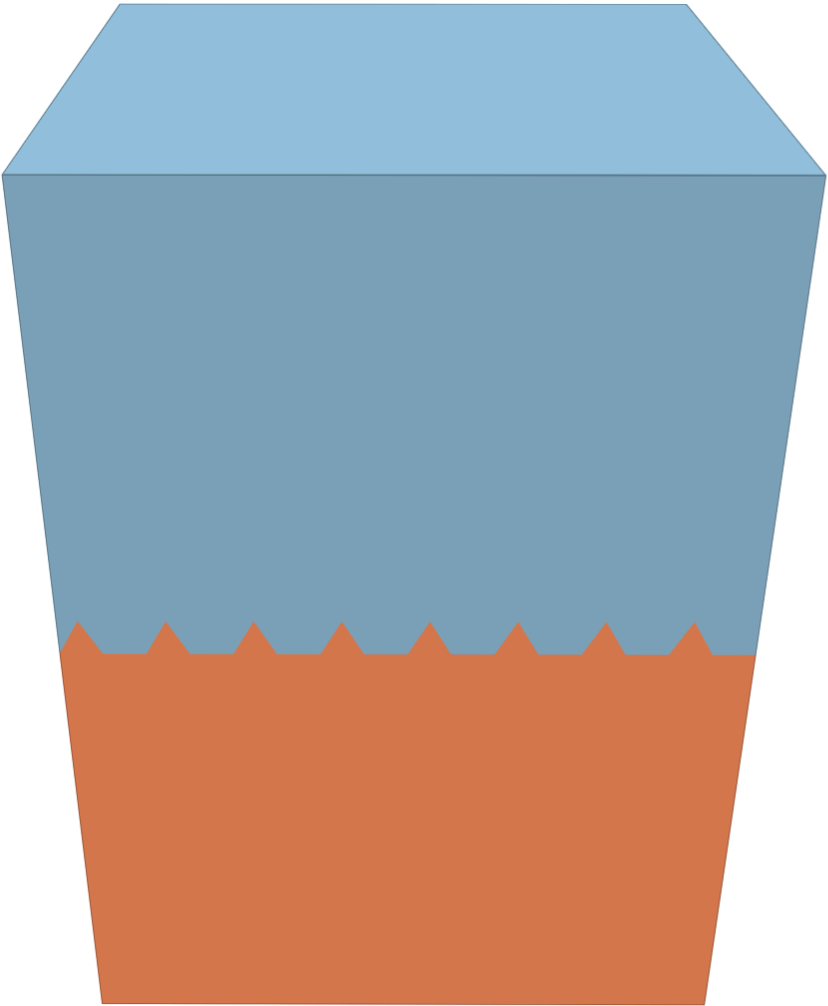
\includegraphics[width=0.15\linewidth]{figures/direction-contour-1}}; &
            \node[anchor=west](double-noise-1) {
                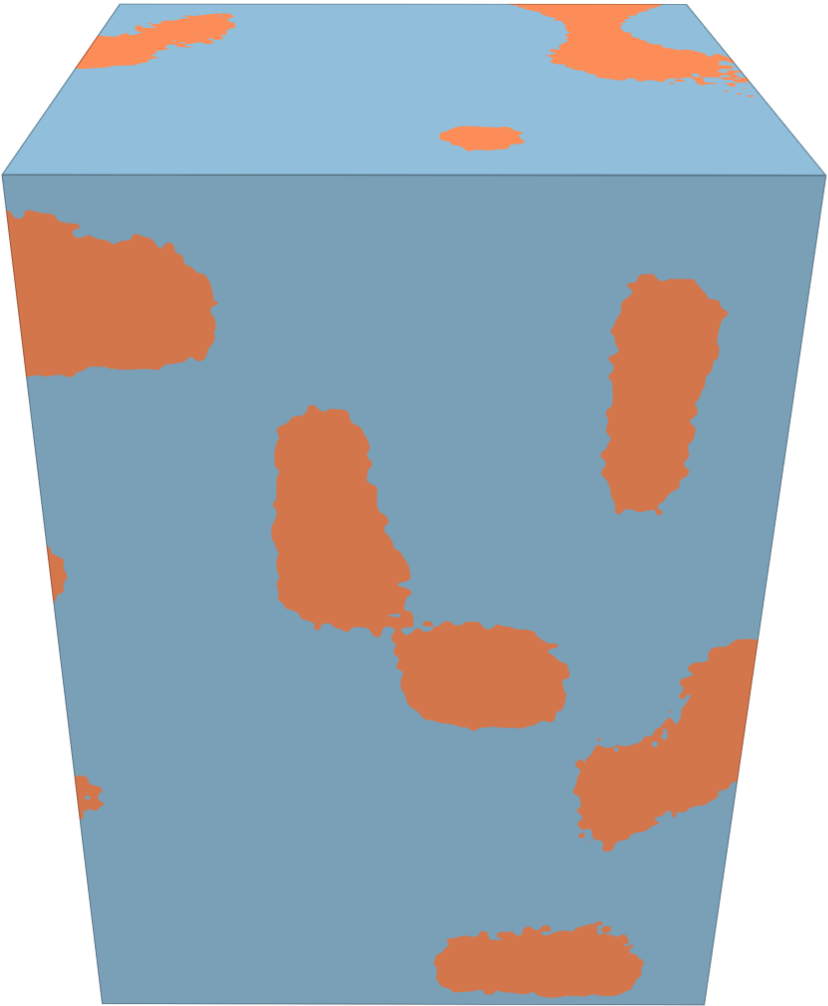
\includegraphics[width=0.15\linewidth]{figures/double-noise-1}}; &
            \node[anchor=west](double-noise-2) {
                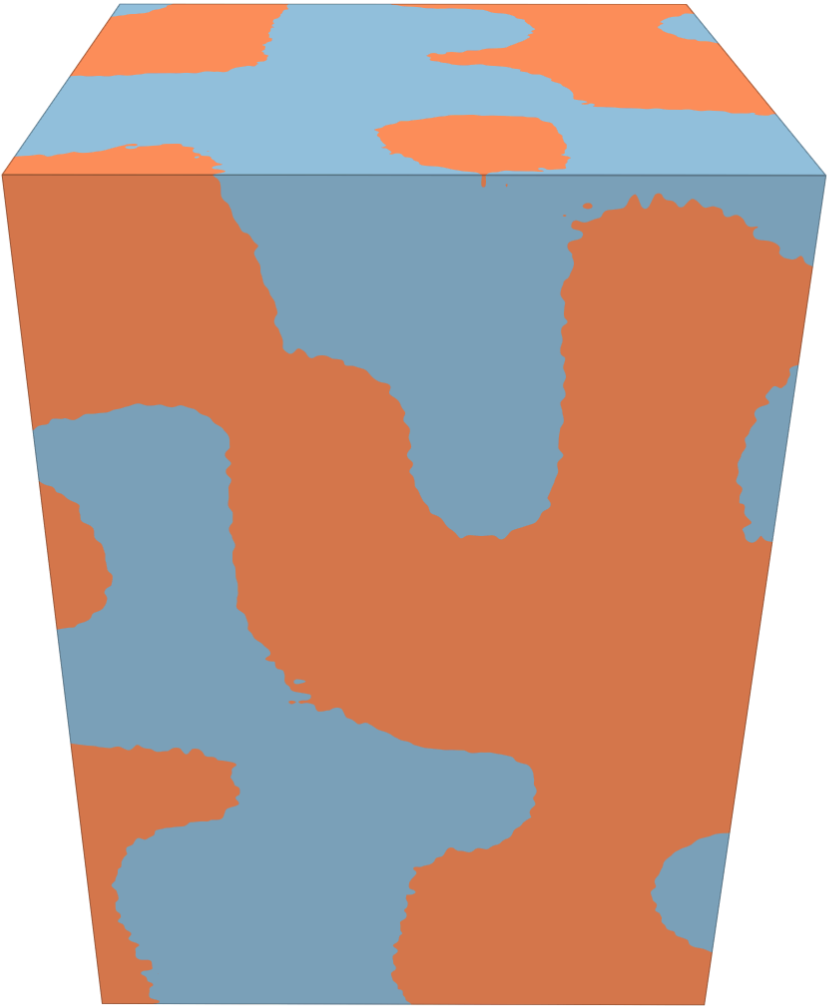
\includegraphics[width=0.15\linewidth]{figures/double-noise-2}}; &
            \node[anchor=west](double-noise-3) {
                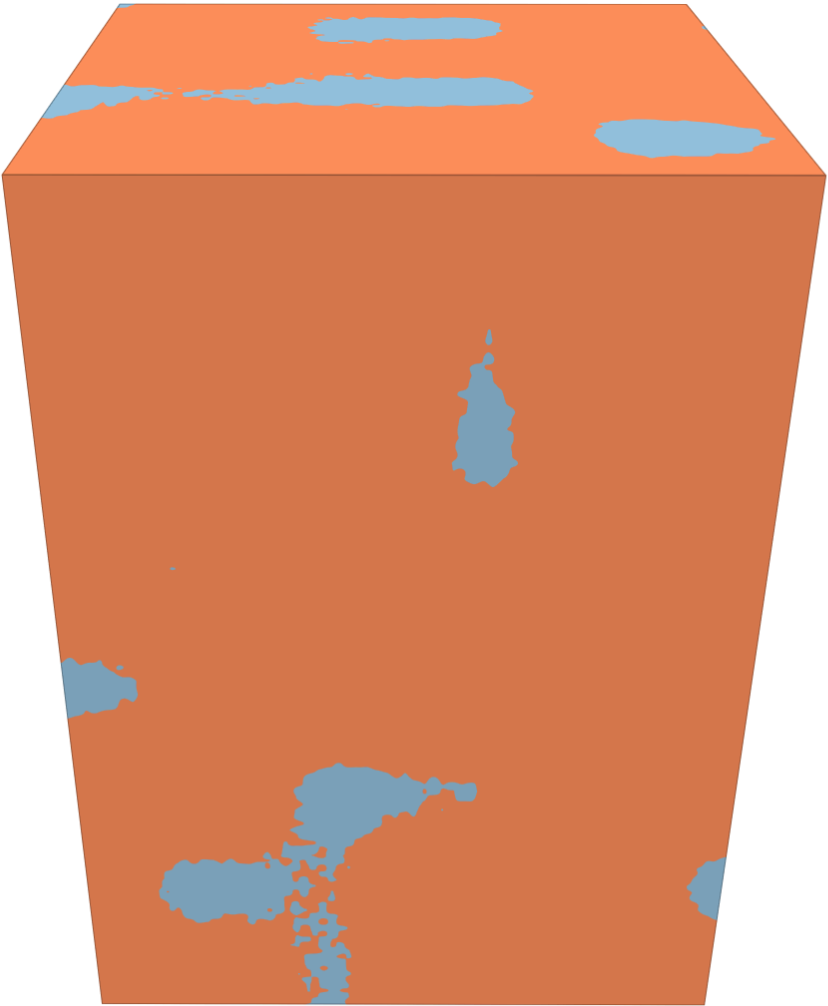
\includegraphics[width=0.15\linewidth]{figures/double-noise-3}};\\
        };
        \draw[dashed,black,shorten >=-12pt,shorten <=-2pt] ($(direction-contour-1.north)!0.5!(double-noise-1.north)$) -- ($(direction-contour-1.south)!0.5!(double-noise-1.south)$) coordinate (label-anchor);
        \node[anchor=north east] at ($(label-anchor)+(-4pt,-4pt)$) { Pillar Pattern + Direction Contour };
        \node[anchor=north west] at ($(label-anchor)+(4pt,-4pt)$) { Noise Pattern + Detail Noise };
        \spy on ($(direction-contour-1)+(+0.25, -0.325)$) in node at ($(-2.0, +0.0)+(direction-contour-1.center)$);
        \spy on ($(double-noise-2.center)+(+0.15, +0.125)$) in node at ($(+4.0, +0.0)+(double-noise-2.center)$);
        \node[above right=1em and 1.25em of double-noise-1.north west,anchor=south east] {$t = $};
        \node[above right=1em and 2em of double-noise-1.north west,anchor=south west] (zero) {0.2};
        \node[above left=1em and 0.5em of double-noise-3.north east,anchor=south east] (one) {0.9};
        \draw[very thin,|-latex,shorten <= 1em,shorten >= 1em] (zero) -- (one);
    \end{tikzpicture}
    \caption{
        Example of two extensions to the proposed Pillar pattern and Noise pattern. The Pillar pattern was extended by a direction contour (left) that uses indents in the border between the two colors resembling arrowheads to encode the animation direction. The Noise pattern was extended with detail noise (right). However, this detail noise does not allow encoding a direction of change.
    }
    \label{fig:extended-examples}
\end{figure}
\paragraph{Implementation.}
Implementing the prototype using hardware-accelerated rendering and procedural texture patterns seems advantageous, as it allows for a broad range of patterns, combinations, and extensions.
Using a pattern as a starting point is straightforward (see \autoref{fig:extended-examples}).
The overhead in rendering times is reasonable and allows for interactive frame rates for mid-scale and even large datasets with hundreds and thousands of nodes.

\section{Conclusions}
We have shown that exploring time-varying, tree-structured data using 3D-embedded treemaps is feasible by means of (and in addition to area, height, and color) transitional visual variables.
When depicting two consecutive states in an in-situ fashion, encoding the direction of change is crucial to decode the visualization with its former and latter state effectively.
We proposed texture patterns that support displaying changes in colors using procedural textures.
Those texture patterns are applicable for static contexts---i.e., static images---, or interactive contexts through interactive clients with navigation and interaction.
For specific templates on how to transition color values in 3D we proposed the seven variants (1) Pillar, (2) Pyramid, (3) Arrows, (4) Arrows (full), (5) Noise, (6) Dithering, and (7) Squares.
We discussed the different characteristics, especially the direction of change in value and the direction of animation, and the strengths and weaknesses of each pattern.
Due to a pending user evaluation, we cannot conclude a default pattern at this point.
Further, the proposed texture patterns are currently not fully compatible with other approaches using procedural textures used to encode the direction of change for spatial changes of cuboids.
The prototype indicates that these procedural texture patterns require little overhead for basic implementations, and interactive framerates are achieved even for large-sized treemaps.

Future work includes quantitative evaluations using comprehensive user studies and extended case studies on large software systems and long periods.
The goal would be to find one pattern or a small set of patterns that perform best regarding readability.
Further, the proposed patterns can be revised and extended, e.g., to support general extruded shapes for 2.5D treemaps and 2.5D information visualization in general.
Another goal is to find combinations of different, independent encodings for the direction of change for areas, heights, and colors.

\section*{Acknowledgments}
We want to thank the anonymous reviewers for their valuable comments and suggestions to improve this article.
This work is part of the \enquote{Software-DNA} project, which is funded by the European Regional Development Fund (ERDF or EFRE in German) and the State of Brandenburg (ILB).
This work is also part of the ZIM project \enquote{TASAM}, which is funded by the German Federal Ministry for Economic Affairs and Energy (BMWi).

\bibliographystyle{spbasic}
\bibliography{references}

\end{document}
